\subsection{Case of coverings associated with a principal covering}

Let B be a topological space, let G be a discrete topological group, and let E be a principal covering of B with group G. Denote by p the projection of the B-space E. Let b be a point of B and let x be a point of \(E_{b}\) .

PROPOSITION 5. --- The map \(h_{(\mathrm{E},x)}\) from \(\pi_1(\mathrm{B},b)\) to G which, to \(\gamma \in \pi_1(\mathrm{B},b)\) , associates the unique element \(g\) of G such that \(x \cdot g = x \cdot \gamma^{-1}\) is a group homomorphism, whose kernel is the subgroup \(p_*(\pi_1(\mathrm{E},x))\) of \(\pi_1(\mathrm{B},b)\) . If E is connected, this homomorphism is surjective.

For every \(g \in \mathrm{G}\) , we have \(h_{(\mathrm{E},x \cdot g)} = \operatorname{Int}(g^{-1}) \circ h_{(\mathrm{E},x)}\) .

Let E be a principal covering of B with group G, let x be a point of \(E_{b}\) and denote by p the projection of E. For every \(g \in G\) , the map \(y \mapsto y \cdot g\) is a B-automorphism of E. We therefore have, for every \(g \in G\) , every \(y \in E_{b}\) and every \(\gamma \in \pi_{1}(B, b)\) , the relation \((y \cdot g) \cdot \gamma = (y \cdot \gamma) \cdot g\) (cf. III, p. 305, relation (4)). Consequently, for \(\gamma, \delta \in \pi_{1}(B, b)\) , we have

\[
\begin{array}{r l} & {x \cdot h _ {(\mathrm{E}, x)} (\gamma \delta) = x \cdot \delta^ {- 1} \gamma^ {- 1}} \\ & {\qquad = (x \cdot h _ {(\mathrm{E}, x)} (\delta)) \cdot \gamma^ {- 1}} \\ & {\qquad = (x \cdot \gamma^ {- 1}) \cdot h _ {(\mathrm{E}, x)} (\delta)} \\ & {\qquad = x \cdot h _ {(\mathrm{E}, x)} (\gamma) h _ {(\mathrm{E}, x)} (\delta),} \end{array}
\]

which proves that \(h_{(\mathrm{E},x)}\) is a group homomorphism.

Its kernel is the stabilizer of \(x\) for the canonical action of \(\pi_1(\mathrm{B}, b)\), and therefore is equal to \(p_*(\pi_1(\mathrm{E}, x))\) by Theorem 1 of III, p. 305. The map \(g \mapsto x \cdot g\) is a bijection from G onto \(\mathrm{E}_b\). The image of the homomorphism \(h_{(\mathrm{E}, x)}\) is therefore the set of \(g \in \mathrm{G}\) such that \(x \cdot g\) belongs to the orbit of \(x\) for this operation. If E is connected, \(\pi_1(\mathrm{B}, b)\) acts transitively on \(\mathrm{E}_b\) (loc. cit.) and the homomorphism \(h_{(\mathrm{E}, x)}\) is surjective.

Let \(g\in \mathbf{G}\) ; for every \(\gamma \in \pi_1(\mathrm{B},b)\) , we have

\[
x \cdot g h _ {(\mathrm{E}, x \cdot g)} (\gamma) = (x \cdot g) \cdot \gamma^ {- 1} = (x \cdot \gamma^ {- 1}) \cdot g = x \cdot h _ {(\mathrm{E}, x)} (\gamma) g,
\]

whence \(h_{(\mathrm{E},x\cdot g)}(\gamma)=g^{-1}h_{(\mathrm{E},x)}(\gamma)g\) . This completes the proof of the proposition.

Examples. --- 1) Let F be a discrete set equipped with an action of G and let \(X = E \times^{G} F\) be the covering of B associated with it. Denote by \(\varphi: E \times F \to X\) the canonical B-morphism. It is a morphism of coverings. For every \(\gamma \in \pi_{1}(B, b)\) and every \(f \in F\) , we then have

\[
\varphi (x, f) \cdot \gamma = \varphi (x \cdot \gamma , f) = \varphi (x \cdot h _ {(\mathrm{E}, x)} (\gamma) ^ {- 1}, f) = \varphi (x, h _ {(\mathrm{E}, x)} (\gamma^ {- 1}) \cdot f).\tag{5}
\]

If one identifies F with \(X_{b}\) by the bijective map \(f \mapsto \varphi(x, f)\) , it follows that the right operation \(\pi_{1}(B, b) \to \operatorname{Aut}(X_{b})^{\circ}\) is the composition of the homomorphism \(h_{(E,x)}\) , the antihomomorphism \(g \mapsto g^{-1}\) of G into itself and the homomorphism G → Aut(F) induced by the action of G on F.

\begin{enumerate}
\def\labelenumi{\arabic{enumi})}
\setcounter{enumi}{1}
\tightlist
\item
  Let H be a discrete topological group, let \(f\colon G\to H\) be a group homomorphism. Endow H with the left action of G given by \(g\cdot h=f(g)h\) , for \(g\in G\) and \(h\in H\) . Let \(\mathrm{E}^{\prime}=\mathrm{E}\times^{\mathrm{G}}\mathrm{H}\) be the associated covering; it is a principal covering with group H (I, p. 107, example 6). Denote by \(q\colon E\times H\to E\times^{G}H\) the canonical map and set \(x^{\prime}=q(x,e)\) . We have \(h_{(E^{\prime},x^{\prime})}=f\circ h_{(E,x)}\) .
\end{enumerate}

Indeed, let \(c\) be a loop at \(b\) in B, let \(\gamma\) be its class in \(\pi_1(B,b)\) and let \(g = h_{(E,x)}(\gamma)\) ; one therefore has \(x \cdot \gamma = x \cdot g^{-1}\) . Let \(\widetilde{c}\) be a path with origin \(x\) in E; then, \(t \mapsto q(\widetilde{c}(t), e)\) is a path with origin \(x'\) in E' which lifts the path \(p \circ \widetilde{c}\) in B, so that

\[
x ^ {\prime} \cdot \gamma = q (x \cdot \gamma , e) = q (x \cdot g ^ {- 1}, e) = q (x, f (g) ^ {- 1}) = q (x, e) \cdot f (g) ^ {- 1},
\]

which proves that \(h_{(\mathrm{E}', x')}(\gamma) = f(g)\) .

\section{HOMOTOPY AND COVERINGS (CASE OF LOCALLY ARC-CONNECTED SPACES)}

\subsection{Homotopy lifting condition for continuous maps}

PROPOSITION 1. --- Let B be a topological space and let (E,p) be a covering of B. Let Y be a topological space and let f: Y → B be a continuous map. Let y ∈ Y, x ∈ E, b ∈ B be points such that f(y) = p(x) = b. Suppose the space Y is connected and locally path-connected. For there to exist a continuous lifting g: Y → E of f such that g(y) = x, it is necessary and sufficient that the image of the homomorphism π₁(f,y): π₁(Y,y) → π₁(B,b) be contained in the image of the homomorphism π₁(p,x): π₁(E,x) → π₁(B,b).

The condition is necessary without any hypothesis on the space Y. Indeed, if such a lifting g exists, we have \(\pi_{1}(f,y)=\pi_{1}(p,x)\circ\pi_{1}(g,y)\) .

Let us prove that it is sufficient. Denote by \(s\colon \Lambda_{b}(\mathrm{B})\to \Lambda_{x}(\mathrm{E})\) the inverse homeomorphism of the homeomorphism \(c\mapsto p\circ c\) (III, p. 302, cor. 2 of prop. 3) and let \(\varphi \colon \Lambda_y(\mathrm{Y})\to \Lambda_x(\mathrm{E})\) be the map \(d\mapsto s(f\circ d)\) . The map \(\varphi\) is continuous (I, p. 132, lemma).

Let \(d\) and \(d' \in \Lambda_y(Y)\) be paths with origin \(y\) having the same term; let us prove that the paths \(\varphi(d)\) and \(\varphi(d')\) have the same term. Set \(c = f \circ d\) , \(c' = f \circ d'\) . Since the path \(d * \overline{d'}\) is a loop in Y at \(y\) , the path \(c * \overline{c'}\) is a loop in B at \(b\) and its class belongs to the image of the homomorphism \(\pi_1(f, y)\) , hence to the image of the homomorphism \(\pi_1(p, x)\) by hypothesis. By cor. 2 of prop. 4 (III, p. 303), the path \(s(c * \overline{c'})\) is a loop in E at \(x\) . The same is true of the path \(s(c' * \overline{c})\) which, by uniqueness of path lifting, is equal to \(\overline{s(c * \overline{c'})}\) . We therefore have \(s(c' * \overline{c})(\frac{1}{2}) = s(c')(1) = s(c)(1)\) , which is what we wanted to prove.

Let us denote respectively by \(e_{\mathrm{E}}\colon\Lambda_{x}(\mathrm{E})\to\mathrm{E}\) and \(e_{\mathrm{Y}}\colon\Lambda_{y}(\mathrm{Y})\to\mathrm{Y}\) the terminal maps. Since the space Y is assumed to be connected and locally path-connected, the map \(e_{Y}\) is surjective and open (III, p. 262, prop. 10). By the preceding paragraph, there exists a unique map \(g\colon Y\to E\) such that \(e_{E}\circ\varphi=g\circ e_{Y}\) . It is continuous, because the map \(e_{Y}\) is strict (I, p. 18, example 2).

Finally, let us verify that the map g lifts the map f and that \(g(y) = x\) . Every point z of Y is the terminal point of a path c with origin y. The path \(\varphi(c)\) is a lifting of \(f \circ c\) with origin x and terminal point \(g(z)\) . We therefore have \(p(g(z)) = f(z)\) . For z = y and \(c = e_y\) , we have \(\varphi(e_y) = e_x\) , whence \(g(y) = x\) .

COROLLARY 1. --- Let B be a connected and locally path-connected topological space, and let b be a point of B. For a covering (E, p) of B to be trivializable, it is necessary and sufficient that, for every point x of the fibre \(E_{b}\) , the homomorphism \(\pi_{1}(p, x)\) be bijective.

Recall that the homomorphism \(\pi_{1}(p,x)\) is injective (III, p. 303, cor. 1 of prop. 4). The statement therefore follows from prop. 1 and I, p. 81, cor. 4 of prop. 6.

Remark. --- Let B be a locally path-connected topological space, let b be a point of B and let V be an open connected neighbourhood of b such that the homomorphism from \(\pi_{1}(V,b)\) to \(\pi_{1}(B,b)\) has as its image the subgroup reduced to the identity element. By cor. 1, every covering of B is trivializable above V, and a fortiori above every subset of B contained in V.

COROLLARY 2. --- Let B be a connected and locally path-connected topological space. If, for a point b of B, the group \(\pi_1(B,b)\) is reduced to the identity element, then the space B is simply connected.

Indeed, it follows from corollary 1 that, under these hypotheses, every covering of B is trivializable.

COROLLARY 3. --- Let

\pandocbounded{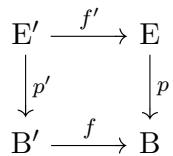
\includegraphics[keepaspectratio]{images/part002_b7191fdb.jpg}}

be a cartesian square. Suppose that E is a covering of B and that the space B' is connected and locally path-connected. Let b' be a point of B' and \(b = f(b')\) . For \((\mathrm{E}', p')\) to be a trivializable covering of B', it is necessary and sufficient that, for every point x of the fibre \(E_b\), the image of \(\pi_1(p, x)\) contain the image of \(\pi_1(f, b)\) .

This follows from prop. 1 and I, p. 81, cor. 5 of prop. 6.

\subsection{Operations of the Poincaré group and morphisms of coverings}

Let B be a connected and locally path-connected topological space and let b be a point of B.

Let E be a covering of B. Since the space B is assumed to be connected, the fibre \(E_{b}\) is nonempty if E is nonempty (I, p. 74, prop. 4). By assertion a) of theorem 1 of III, p. 305, the covering E is connected and nonempty if and only if the group \(\pi_{1}(B,b)\) acts transitively on \(E_{b}\) .

PROPOSITION 2. --- Let E and E' be coverings of B.

\begin{enumerate}
\def\labelenumi{\alph{enumi})}
\item
  Let \(f\colon\mathrm{E}\to\mathrm{E}^{\prime}\) be a B-morphism. The map \(f_{b}\colon\mathrm{E}_{b}\to\mathrm{E}_{b}^{\prime}\) deduced from \(f\) is compatible with the operations of \(\pi_{1}(\mathrm{B},b)\) on \(\mathrm{E}_{b}\) and \(\mathrm{E}_{b}^{\prime}\) respectively. It is bijective if and only if \(f\) is an isomorphism.
\item
  The map \(f\mapsto f_{b}\) is a bijection from the set \(\mathcal{C}_{\mathrm{B}}(\mathrm{E};\mathrm{E}^{\prime})\) of B-morphisms from E to \(\mathrm{E}^{\prime}\) onto the set \(\mathcal{F}_{\pi_1(\mathrm{B},b)}(\mathrm{E}_b;\mathrm{E}_b^{\prime})\) of \(\pi_1(\mathrm{B},b)\)-morphisms from \(\mathrm{E}_b\) to \(\mathrm{E}_b^{\prime}\) .
\end{enumerate}

If \(f\) is a B-morphism from E to \(\mathrm{E}'\) , the map \(f_b\colon \mathrm{E}_b\to \mathrm{E}_b'\) is a \(\pi_1(\mathrm{B},b)\) -morphism (cf. III, p. 305). Moreover, two B-morphisms from E to \(\mathrm{E}'\) which coincide on the fibre \(\mathrm{E}_b\) are equal (I, p. 80, cor. 3 of prop. 6).

Let \(\varphi\colon\mathrm{E}_{b}\to\mathrm{E}_{b}^{\prime}\) be a morphism of \(\pi_{1}(\mathrm{B},b)\)-sets; let us show that there exists a B-morphism \(f\) from E to \(\mathrm{E}^{\prime}\) such that \(f_{b}=\varphi\) . We may assume the spaces E and \(\mathrm{E}^{\prime}\) are connected and nonempty, so that \(\mathrm{E}_{b}\) and \(\mathrm{E}_{b}^{\prime}\) are homogeneous \(\pi_{1}(\mathrm{B},b)\)-sets. Let \(x\) be a point of \(\mathrm{E}_{b}\) ; its stabilizer G is the image of the map \(\pi_{1}(p,x)\) (III, p. 305, Theorem 1). Since the map \(\varphi\) is a \(\pi_{1}(\mathrm{B},b)\)-morphism, the group G fixes the point \(x^{\prime}=\varphi(x)\) of \(\mathrm{E}_{b}^{\prime}\) , hence is contained in the image of the map \(\pi_{1}(p^{\prime},x^{\prime})\) . By Prop. 1 of III, p. 308, there exists a B-morphism \(f\) from E to \(\mathrm{E}^{\prime}\) such that \(f(x)=x^{\prime}\) . The maps \(f_{b}\) and \(\varphi\) are \(\pi_{1}(\mathrm{B},b)\)-morphisms of the homogeneous \(\pi_{1}(\mathrm{B},b)\)-set \(\mathrm{E}_{b}\) to \(\mathrm{E}_{b}^{\prime}\) which coincide at the point \(x\) ; they are therefore equal.

If \(f\colon \mathrm{E}\to \mathrm{E}'\) is a B-isomorphism, the map \(f_{b}\colon \mathrm{E}_{b}\to \mathrm{E}_{b}^{\prime}\) is bijective. Conversely, suppose the map \(f_{b}\) is bijective and let \(g\colon \mathrm{E}^{\prime}\to \mathrm{E}\) be a B-morphism such that \(g_{b} = (f_{b})^{-1}\) . The B-morphism \(g\circ f\colon \mathrm{E}\to \mathrm{E}\) induces on \(\mathrm{E}_b\) the identity map; it therefore follows from the proposition that \(g \circ f = Id_{E}\) . Likewise, \(f \circ g = Id_{E'}\) , which proves that f is a B-isomorphism.

COROLLARY 1. --- The coverings E and E' are isomorphic if and only if the \(\pi_1(\mathrm{B},b)\) -sets \(\mathrm{E}_b\) and \(\mathrm{E}_b'\) are isomorphic.

COROLLARY 2. --- Let (E,p) and (E',p') be connected coverings of B. Let \(x\) be a point of \(E_{b}\) and \(x'\) a point of \(E'_{b}\) . For there to exist a B-morphism \(g\colon E\to E'\) such that \(g(x)=x'\), it is necessary and sufficient that \(p_{*}(\pi_{1}(E,x))\subset p'_{*}(\pi_{1}(E',x'))\). Such a morphism is then unique and is an isomorphism if and only if the subgroups \(p_{*}(\pi_{1}(E,x))\) and \(p'_{*}(\pi_{1}(E',x'))\) of \(\pi_{1}(B,b)\) are equal.

By III, p. 305, Theorem 1, the map from \(\pi_1(B,b)\) onto \(E_b\) defined by \(\gamma \mapsto x \cdot \gamma\) induces by passage to the quotient an isomorphism of the \(\pi_1(B,b)\)-set \(p_*(\pi_1(E,x)) \backslash \pi_1(B,b)\) onto \(E_b\) . Likewise, there exists a unique isomorphism of \(\pi_1(B,b)\)-sets from \(p'_{*}(\pi_1(E',x')) \backslash \pi_1(B,b)\) onto \(E_b'\) . By Proposition 2, there exists a B-morphism \(g\colon E\to E'\) such that \(g(x)=x'\) if and only if there exists a morphism of \(\pi_1(B,b)\)-sets from \(p_*(\pi_1(E,x)) \backslash \pi_1(B,b)\) onto \(p'_{*}(\pi_1(E',x')) \backslash \pi_1(B,b)\) sending the class \(p_*(\pi_1(E,x))\) to the class \(p'_{*}(\pi_1(E',x'))\) . Such a morphism exists if and only if one has \(p_*(\pi_1(E,x)) \subset p'_{*}(\pi_1(E',x'))\) . It is then unique, since the space E is assumed connected (I, p. 34, Cor. 2 of Prop. 11). It is an isomorphism if and only if the subgroups \(p_*(\pi_1(E,x))\) and \(p'_{*}(\pi_1(E',x'))\) of \(\pi_1(B,b)\) are equal.

COROLLARY 3. --- Let (E,p) be a connected covering of B and let x be a point of the fiber \(E_{b}\) . Let N denote the normalizer of \(p_{*}(\pi_{1}(E,x))\) in \(\pi_{1}(B,b)\) . For every element \(\gamma\) of N, there exists a unique B-automorphism g of E such that \(g(x) = x \cdot \gamma\) , and the map \(\gamma \mapsto g\) defines by passage to the quotient a group isomorphism from \(\mathrm{N}/p_{*}(\pi_{1}(\mathrm{E},x))\) onto \(\mathrm{Aut}_{\mathrm{B}}(\mathrm{E})\) .

Let \(\gamma \in \pi_1(\mathrm{B}, b)\) ; we have \(p_*(\pi_1(\mathrm{E}, x)) = \operatorname{Int}(\gamma)(p_*(\pi_1(\mathrm{E}, x \cdot \gamma)))\) (III, p. 305, Theorem 1, c)). By Corollary 2, for there to exist a B-automorphism \(g\) of E such that \(g(x) = x \cdot \gamma\) , it is necessary and sufficient that \(\gamma\) belongs to N. Such an isomorphism is then unique. Let us denote by \(\alpha: \mathrm{N} \to \mathrm{Aut}_{\mathrm{B}}(\mathrm{E})\) the map \(\gamma \mapsto g\) thus defined.

Let \(\gamma\) and \(\gamma'\) be two elements of N. Set \(g = \alpha(\gamma)\) , \(g' = \alpha(\gamma')\) ; we have \(g(g'(x)) = g(x \cdot \gamma') = g(x) \cdot \gamma' = (x \cdot \gamma) \cdot \gamma' = x \cdot (\gamma\gamma')\) by relations (4), III, p. 305 and (1), p. 304. Consequently, \(\alpha\) is a group homomorphism. For \(\alpha(\gamma) = \mathrm{Id}_{\mathrm{E}}\) , it is necessary and sufficient that one have \(x \cdot \gamma = x\) , by virtue of the uniqueness of \(\alpha(\gamma)\) , that is, \(\gamma \in p_*(\pi_1(E, x))\) (III, p. 305, Theorem 1, b)). Finally, if \(g\) is a B-automorphism of E, there exists a path \(c\) joining \(x\) to \(g(x)\) in E (which is path-connected), and one then has \(g(x) = x \cdot \gamma\) , where \(\gamma\) is the class of the path \(p \circ c\) . This proves that the homomorphism \(\alpha\) is surjective.

The group \(\mathrm{Aut}_{\mathrm{B}}(\mathrm{E})\) acts on the fibre \(\mathrm{E}_b\) and is identified with the group of automorphisms of the homogeneous \(\pi_1(\mathrm{B},b)\) -set (on the right) \(\mathrm{E}_b\) (cf. A, I, p. 56, prop. 5 and 6).

COROLLARY 4. --- Let (E, p) be a connected covering of B and let x be a point of the fibre \(E_{b}\) . For E to be a Galois covering of B, it is necessary and sufficient that \(p_{*}(\pi_{1}(E, x))\) be a distinguished subgroup of \(\pi_{1}(B, b)\) . The group \(\mathrm{Aut}_{\mathrm{B}}(\mathrm{E})\) is then isomorphic to the quotient group \(\pi_{1}(\mathrm{B}, b)/p_{*}(\pi_{1}(\mathrm{E}, x))\) .

If \(p_{*}(\pi_{1}(\mathrm{E},x))\) is a distinguished subgroup of \(\pi_1(\mathrm{B},b)\) , the group \(\mathrm{Aut}_{\mathrm{B}}(\mathrm{E})\) acts transitively on the fibre \(\mathrm{E}_b\) by Corollary 3, so that E is a Galois covering of B (I, p. 102, th. 2). The converse is assertion d) of Theorem 1 (III, p. 305). The last assertion follows from Corollary 3.

\subsection{Operations without local monodromy of the Poincaré groupoid}

Lemma 1. --- Let B be a locally arcwise connected topological space, let \(p \colon E \to B\) and \(p' \colon E' \to B\) be étale and separated maps satisfying the path lifting property (III, p. 302). Let \(g \colon E \to E'\) be a mapping such that \(p' \circ g = p\) . We assume that \(g\) is compatible with the canonical operations of the groupoid \(\varpi(B)\) on \(E\) and \(E'\) . Then, \(g\) is continuous.

Let c be a path in E; set \(c' = g \circ c\) and let us prove that the map \(c'\) is continuous. Let d denote the path \(p \circ c\) in B and, for every \(t \in I\) , denote by \(d_t\) the path \(s \mapsto d(st)\) . For all \(t \in I\) , we have \(c(t) = c(0) \cdot d_t\) (III, p. 304, remark 3), whence \(c'(t) = c'(0) \cdot d_t\) by the hypothesis made on g, which proves that \(c'\) is a path lifting the path d, by this same remark. This proves that the map g is continuous by arcs. Since the space E is locally arc-connected (III, p. 261, cor. 2), the map g is continuous (III, p. 269, corollary of prop. 13).

Let B be a topological space. Consider an operation \(\varphi = (\varphi_{a,b})_{(a,b)\in \mathrm{B}\times \mathrm{B}}\) of the groupoid \(\varpi (\mathrm{B})\) on a set E, with respect to a mapping \(p\colon \mathrm{E}\to \mathrm{B}\) . One says that \(\varpi (\mathrm{B})\) acts without monodromy on E (cf. II, p. 168) if for every \(b\in \mathrm{B}\) and every loop class \(\gamma \in \pi_1(\mathrm{B},b)\) the action of \(\gamma\) on the fiber \(\mathrm{E}_b\) is trivial. If B is path-connected, it suffices that this be the case for one point of B (loc. cit.). We shall say that the operation \(\varphi\) of the groupoid \(\varpi (\mathrm{B})\) is without local monodromy if every point of B has a neighborhood V such that \(\varpi (\mathrm{V})\) acts without monodromy on the set \(\mathrm{E_V} = p^{-1}(\mathrm{V})\) with respect to the map \(p_{\mathrm{V}} = p\mid p^{-1}(\mathrm{V})\) .

Remark. --- Let B be a locally path-connected topological space, and suppose that every point b of B has a neighborhood V such that the image of \(\pi_{1}(V,b)\) in \(\pi_{1}(B,b)\) is reduced to the identity element (cf. IV, p. 340, def. 2). Then, every operation of the groupoid \(\varpi(B)\) is without local monodromy.

Indeed, consider a set E, a mapping \(p \colon \mathrm{E} \to \mathrm{B}\) and an operation \(\varphi\) of the groupoid \(\varpi(\mathrm{B})\) on E with respect to \(p\) . Let \(a\) be a point of B, and let V be a neighborhood of \(a\) such that the image of \(\pi_1(\mathrm{V}, a)\) in \(\pi_1(\mathrm{B}, a)\) is reduced to the identity element. Let U be a path-connected neighborhood of \(a\) contained in V. Let \(b\) be a point of U and let \(\gamma \in \pi_1(\mathrm{U}, b)\) . Let \(\delta\) be the class of a path joining \(a\) to \(b\) in U. Then, \(\delta\gamma\delta^{-1}\) is the class of a loop at \(a\) in U; its image in \(\pi_1(\mathrm{B}, a)\) is therefore trivial. We thus have \(\varphi_{a,a}(\delta\gamma\delta^{-1}) = \mathrm{Id}_{\mathrm{E}_a}\) , whence \(\varphi_{b,b}(\gamma) = \mathrm{Id}_{\mathrm{E}_b}\) . This proves that the operation of \(\varpi(\mathrm{U})\) on the U-space \(\mathrm{E_U}\) is without monodromy. Consequently, the operation \(\varphi\) is without local monodromy.

PROPOSITION 3. --- Let B be a locally path-connected topological space and let E be a set equipped with an operation \(\varphi\) of the groupoid \(\varpi(B)\), without local monodromy, relative to a mapping \(p: E \to B\). There then exists on E a unique topology for which the following conditions are satisfied:

\begin{enumerate}
\def\labelenumi{(\roman{enumi})}
\item
  The set E equipped with this topology and with the map p is a covering of B;
\item
  The canonical action of \(\varpi(\mathrm{B})\) on this covering is identical to the action \(\varphi\) .
\end{enumerate}

The uniqueness of such a topology follows from lemma 1 of III, p. 312, where one takes for g the identity map of E. To prove its existence, one may moreover assume that B is connected and nonempty.

Suppose first that the operation \(\varphi = (\varphi_{a,b})_{(a,b)\in \mathrm{B}\times \mathrm{B}}\) of the groupoid \(\varpi (\mathrm{B})\) on the set E, relative to \(p\) , is without monodromy.

Let \(a\) be a point of B. For every point \(b \in \mathrm{B}\) , there exists a path \(c\) in B joining \(a\) to \(b\) . If \(\gamma \in \varpi_{a,b}(\mathrm{B})\) denotes the class of the path \(c\) , the bijection \(\varphi_{a,b}(\gamma) \colon \mathrm{E}_a \to \mathrm{E}_b\) is independent of the path \(c\) , since the operation is without monodromy; we denote by \(f_{a,b}\) this bijection. The map \(\Phi_a \colon \mathrm{B} \times \mathrm{E}_a \to \mathrm{E}\) defined by \((b,x) \mapsto f_{a,b}(x)\) is a bijection; the inverse bijection maps \(x \in \mathrm{E}\) to the pair \((p(x), f_{p(x),a}(x))\) . Endow the set \(\mathrm{E}_a\) with the discrete topology, so that the B-space \(\mathrm{B} \times \mathrm{E}_a\) is a trivial covering of B. By transport of structure, the bijection \(\Phi_a\) endows E with a topology making it a covering of B.

Let us prove that the canonical operation of \(\varpi(\mathrm{B})\) on E is identical to the operation \(\varphi\) . Let \(x\) be a point of \(\mathrm{E}_a\) and \(b\) a point of B. Let \(c\) be a path in B joining the point \(a\) to the point \(b\) ; the map \(t \mapsto \Phi_a(c(t), x)\) is then a path in E joining the point \(x\) to the point \(\Phi_a(b, x) = f_{a,b}(x)\) . If \(\gamma \in \varpi_{a,b}(\mathrm{B})\) denotes the class of the path \(c\) , we thus have \(x \cdot \gamma = f_{a,b}(x)\) . This shows that the canonical action of \(\varpi(\mathrm{B})\) on the covering E and the operation \(\varphi\) coincide on the classes of paths of origin \(a\) . Since these classes generate the groupoid \(\varpi(\mathrm{B})\) , the two operations are equal.

Now let us treat the general case. Let \(\mathcal{B}\) be the set of open subsets V of E such that \(\varpi(\mathrm{V})\) acts without monodromy on \(p^{-1}(\mathrm{V})\) . By hypothesis, the elements of \(\mathcal{B}\) cover B. By the preceding, there exists for every \(\mathrm{V} \in \mathcal{B}\) a unique topology on the set \(p^{-1}(\mathrm{V})\) such that \((p^{-1}(\mathrm{V}), p_{\mathrm{V}})\) makes it a covering of V and such that the canonical action of \(\varpi(\mathrm{V})\) on this covering coincides with the action induced by \(\varphi\) .

Let V and \(V' \in \mathcal{B}\) . The topology of \(p^{-1}(V \cap V')\) induced by the topology of \(p^{-1}(V)\) (resp. of \(p^{-1}(V')\) ) defined above indeed makes a covering of \(V \cap V'\) on which the canonical operation of \(\varpi(V \cap V')\) is induced by the operation \(\varphi\) . These topologies therefore coincide with that of \(p^{-1}(V \cap V')\) . There then exists a unique topology on E inducing on each \(p^{-1}(V)\) the topology previously defined (cf. I, §2, p. 16).

When E is equipped with this topology, the map p is continuous and the B-space E is a covering. The canonical action of \(\varpi(\mathrm{B})\) on this covering coincides with the operation \(\varphi\) on the classes of paths whose image is contained in one of the open sets of \(\mathcal{B}\) . By Lemma 4 of

III, p. 272, these classes generate the groupoid \(\varpi(B)\) . It follows that these two operations are equal (II, p. 167).

COROLLARY. --- Let B be a connected and locally arcwise connected topological space, let (E,p) be a B-space whose projection p is étale, separated, and has the path lifting property. If the canonical operation of \(\varpi(\mathrm{B})\) on the set E, relative to p, is without local monodromy, then E is a covering of B.

Endow E with the canonical action of \(\varpi(B)\) defined by the lifting of paths (III, p. 303, no. 3). There exists a topology on E for which conditions (i) and (ii) of Prop. 3 are satisfied. This topology coincides with the given topology on E by Lemma 1 of III, p. 312.

\subsection{Admissible topology of Poincaré groups}

Let B be a topological space and let \(a\) be a point of B. We say that a subgroup H of \(\pi_1(B, a)\) is admissible if every point \(b\) of B has a neighborhood V such that \(\gamma i_*(\delta)\gamma^{-1} \in \mathrm{H}\) for every \(\gamma \in \varpi_{a,b}(\mathrm{B})\) and every \(\delta \in \pi_1(V, b)\) , where \(i: V \to B\) is the canonical injection. If H is a normal subgroup of \(\pi_1(B, a)\) , it suffices, for H to be admissible, that this condition be verified for one path class \(\gamma \in \varpi_{a,b}(\mathrm{B})\) .

Proposition 4. — There exists a unique topology on \(\pi_1(B, a)\) compatible with its group structure, for which the admissible distinguished subgroups of \(\pi_1(B, a)\) form a fundamental system of neighborhoods of the identity element. For this topology, the open subgroups are exactly the admissible subgroups.

The following facts result from the definition of an admissible subgroup:

\begin{enumerate}
\def\labelenumi{\alph{enumi})}
\item
  The group \(\pi_1(B, a)\) is admissible;
\item
  A subgroup containing an admissible subgroup is admissible;
\item
  The intersection of a finite family of admissible subgroups is admissible.
\item
  For every admissible subgroup H of \(\pi_{1}(B,a)\) the intersection of the subgroups \(\gamma H\gamma^{-1}\) , when \(\gamma\) runs through \(\pi_{1}(B,a)\) , is admissible.
\end{enumerate}

In particular, the set of admissible normal subgroups is a filter base consisting of subgroups of \(\pi_1(B,a)\) satisfying the axiom (GV \(_{\text{III}}'\) ) of III, p. 4, whence the first part of the proposition according to TG, III, p. 5, example. The second part is then immediate (cf. TG, III, p. 7, corollary of prop. 4).

The topology on the group \(\pi_{1}(B,a)\) characterized in Proposition 4 is called the admissible topology.

Remarks. --- 1) If B \(_{0}\) denotes the arcwise connected component of \(a\) in B, the canonical isomorphism \(\pi_{1}(B_{0}, a) \to \pi_{1}(B, a)\) is an isomorphism of topological groups when these groups are equipped with the admissible topology.

\begin{enumerate}
\def\labelenumi{\arabic{enumi})}
\setcounter{enumi}{1}
\item
  Let B be a topological space. Let \(b\) and \(b'\) be points of B belonging to the same path-connected component, and let \(\gamma\) be an element of \(\varpi_{b,b'}(B)\) . It follows from the definition of an admissible subgroup that, for every admissible subgroup H of \(\pi_1(B,b')\) , the subgroup \(\gamma H\gamma^{-1}\) of \(\pi_1(B,b)\) is admissible. Consequently, the isomorphism \(u_\gamma \colon \delta \mapsto \gamma \delta \gamma^{-1}\) of \(\pi_1(B,b')\) onto \(\pi_1(B,b)\) (cf. III, p. 292) is a homeomorphism when these groups are equipped with the admissible topologies.
\item
  Let A and B be topological spaces, let \(a\) be a point of A and let \(f\colon\mathrm{A}\to\mathrm{B}\) be a continuous map. Set \(b=f(a)\) . If H is an admissible subgroup of \(\pi_{1}(\mathrm{B},b)\) , its inverse image under the homomorphism \(\pi_{1}(f,a)\) is an admissible subgroup of \(\pi_{1}(\mathrm{A},a)\) . Consequently, the group homomorphism \(\pi_{1}(f,a)\colon\pi_{1}(\mathrm{A},a)\to\pi_{1}(\mathrm{B},b)\) is continuous, when these groups are equipped with the admissible topology.
\end{enumerate}

PROPOSITION 5. --- Let B be a locally path-connected topological space and let a be a point of B. For a subgroup H of \(\pi_1(\mathrm{B},a)\) to be admissible, it is necessary and sufficient that there exist a covering (E,p) of B and a point \(x\in \mathrm{E}_a\) such that \(\mathrm{H} = p_{*}(\pi_{1}(\mathrm{E},x))\) .

Let \((\mathrm{E},p)\) be a covering of B and let x be a point of \(E_{a}\) ; set \(\mathrm{H}=p_{*}(\pi_{1}(\mathrm{E},x))\) and let us show that it is an admissible subgroup of \(\pi_{1}(\mathrm{B},a)\) . Let b be a point of B and let V be a neighborhood of b such that \(\mathrm{E}_{\mathrm{V}}=(p^{-1}(\mathrm{V}),p_{\mathrm{V}})\) is a trivializable covering of V. Let \(\gamma\in\varpi_{a,b}(\mathrm{B})\) ; we shall prove that for every element \(\delta\in\pi_{1}(\mathrm{V},b)\) , the path class \(\gamma\delta\gamma^{-1}\) belongs to H.

By III, p. 301, prop. 3, there exists a unique strict homotopy class \(\gamma'\) of a path with origin \(x\) in E such that \(p_*(\gamma') = \gamma\) . Let \(y\) be the terminal point of \(\gamma'\) ; we have \(p(y) = b\) (III, p. 302, prop. 4). Let then \(\delta'\) be the unique path class with origin \(y\) in E such that \(p_*(\delta') = \delta\) . Since \(\mathrm{E_V}\) is trivializable, \(\delta'\) is the class of a loop at \(y\) . Then, \(\gamma'\delta'(\gamma')^{-1}\) is the class of a loop at \(a\) in E whose image under \(p_*\) is the class \(\gamma\delta\gamma^{-1}\) , which is what had to be proved.

Conversely, let H be an admissible subgroup of \(\pi_1(B, a)\) . Let \(\lambda_a(B)\) be the quotient of the space \(\Lambda_a(B)\) of paths with origin \(a\) for the strict homotopy relation; since two strictly homotopic paths have the same endpoint, the endpoint map \(e: \Lambda_a(B) \to B\) defines by passage to the quotient a map \(\varepsilon: \lambda_a(B) \to B\) . The composition of path classes endows the set \(\lambda_a(B)\) with a left action of the group \(\pi_1(B, a)\) . Equip it with the action of the group H obtained by restriction, and denote by \(H\backslash\lambda_a(B)\) the set of its orbits.

The map \(\varepsilon\colon\lambda_{a}(B)\to B\) induces, by passing to the quotient, a map \(q\colon H\backslash\lambda_{a}(B)\to B\) . The composition of path classes endows the set \(H\backslash\lambda_a(B)\) with a right action of the groupoid \(\varpi(B)\) with respect to the map \(q\) .

This operation has no local monodromy. Indeed, let \(b\) be a point of B, and let V be a neighborhood of \(b\) such that \(\gamma i_{*}(\pi_{1}(V,b))\gamma^{-1}\subset H\) for every path class \(\gamma\) connecting \(a\) to \(b\) in B, where \(i\) denotes the inclusion of V into B. Since B is locally path-connected, one may further assume that V is path-connected. Let \(c\in V\) , let \(\delta\) be the class in \(\pi_1(B,c)\) of a loop at \(c\) contained in V, and let \(\delta'\) be an element of \(\lambda_a(B)\) such that \(\varepsilon (\delta ') = c\) . Let \(\delta''\) be an element of \(\varpi_{c,b}(V)\) and let us set \(\gamma = \delta '\delta ''\) . By definition of V, the element \(\delta '\delta (\delta ')^{-1} = \gamma ((\delta '')^{-1}\delta \delta '')\gamma^{-1}\) of \(\pi_1(B,a)\) belongs to H. Then, \(\mathrm{H}\delta^{\prime}\cdot \delta = \mathrm{H}\delta^{\prime}\) ; this proves that \(\pi_1(V,c)\) acts trivially on the set \(q^{-1}(c)\) .

By III, p. 313, prop. 3, there exists a unique topology on \(\mathrm{H}\backslash\lambda_{a}(\mathrm{B})\) for which \(q\) is continuous and the B-space \((\mathrm{H}\backslash\lambda_{a}(\mathrm{B}),q)\) is a covering such that the canonical action of \(\varpi(\mathrm{B})\) on this covering is the action defined above. By assertion b) of Theorem 1 of III, p. 305, the group \(q_{*}(\pi_{1}(\mathrm{H}\backslash\lambda_{a}(\mathrm{B}),\mathrm{H}))\) is equal to H.

We will say that an operation of the group \(\pi_1(B, b)\) on a set X is admissible if the kernel of the canonical map \(\pi_1(B, b) \to \mathfrak{S}_{\mathrm{X}}\) is an open subgroup of \(\pi_1(B, b)\) . This amounts to saying that the homomorphism \(\pi_1(B, b) \to \mathfrak{S}_{\mathrm{X}}\) is continuous if the group \(\mathfrak{S}_{\mathrm{X}}\) is equipped with the discrete topology. The map \(\pi_1(B, b) \times X \to X\) is then continuous, when X is endowed with the discrete topology. Conversely, consider a continuous action of \(\pi_{1}(B,b)\) on a discrete space X. Let x be a point of X; its stabilizer is an open subgroup H of \(\pi_{1}(B,b)\) by hypothesis. For \(\gamma\in\pi_{1}(B,b)\) the fixator of \(\gamma\cdot x\) is the subgroup \(\gamma H\gamma^{-1}\) , so that the subgroup of \(\pi_{1}(B,b)\) fixing each element of the orbit of x is the intersection of the subgroups \(\gamma H\gamma^{-1}\) , for \(\gamma\) running through \(\pi_{1}(B,b)\) . It is an open subgroup because the distinguished open subgroups of \(\pi_{1}(B,b)\) form a basis for its topology (III, p. 315, prop. 4). This implies that a continuous action of \(\pi_{1}(B,b)\) on a discrete space X is admissible if it is transitive or, more generally, if the set of orbits of the elements of X is finite.

For any discrete group \(G\), any principal \(G\)-covering \(E\) over \(B\), and any point \(x \in E_{b}\) , recall that the map \(h_{(\mathrm{E},x)}\) from \(\pi_{1}(\mathrm{B},b)\) to G which, to \(\gamma \in \pi_{1}(\mathrm{B},b)\) , associates the unique element \(g \in G\) such that \(x \cdot g = x \cdot \gamma^{-1}\) is a group homomorphism (III, p. 306, prop. 5).

PROPOSITION 6. --- Let B be a topological space and let b be a point of B. Endow the group \(\pi_1(B, b)\) with the admissible topology.

\begin{enumerate}
\def\labelenumi{\alph{enumi})}
\item
  For any discrete group G, any principal covering E of B with group G, and any \(x \in E_{b}\) , the homomorphism \(h_{(E,x)}\) is a continuous homomorphism of topological groups.
\item
  For every covering E of B, the canonical action of \(\pi_{1}(B,b)\) on the fiber \(E_{b}\) is admissible.
\end{enumerate}

It suffices to prove the second assertion. Let K be the set of elements \(k \in \pi_{1}(B, b)\) such that \(x \cdot k = x\) for all \(x \in E_{b}\) . Let us prove that K is an admissible subgroup of \(\pi_{1}(B, b)\) .

Let \(b'\) be a point of B and let \(V'\) be a neighborhood of \(b'\) in B above which the covering E is trivializable. Let \(\gamma\) be the class of a path c connecting \(b\) to \(b'\) in B and let \(c'\) be the unique path starting at x in E that lifts c. For all \(\delta \in \pi_1(V', b')\) and every \(x' \in E_{b'}\) , we have \(x' \cdot \delta = x'\) . Consequently, for \(x \in E_b\) and \(\delta \in \pi_1(V', b')\) , we have

\[
x \cdot \gamma \delta \gamma^ {- 1} = ((x \cdot \gamma) \cdot \delta) \cdot \gamma^ {- 1} = (x \cdot \gamma) \cdot \gamma^ {- 1} = x,
\]

so that \(\gamma\delta\gamma^{-1}\) belongs to K. In other words, K is an admissible subgroup, whence the proposition.

PROPOSITION 7. --- Let B be a connected and locally path-connected topological space, and let b be a point of B. Endow the group \(\pi_1(B, b)\) with the admissible topology.

\begin{enumerate}
\def\labelenumi{\alph{enumi})}
\item
  Let G be a discrete topological group. For every continuous homomorphism \(f\colon \pi_{1}(\mathrm{B},b)\to \mathrm{G}\) , there exists a principal covering E of B with group G, and a point \(x\) of \(\mathrm{E}_{b}\) such that \(h_{(\mathrm{E},x)} = f\) .
\item
  For every discrete topological space F equipped with an admissible right action of the group \(\pi_{1}(B,b)\), there exists a covering E of B such that the \(\pi_{1}(B,b)\)-sets F and \(E_{b}\) are isomorphic.
\end{enumerate}

Let us prove \(a\) ). Let \(f\) be a continuous homomorphism of \(\pi_1(B, b)\) into a discrete group G. Its kernel is an open normal subgroup K of \(\pi_1(B, b)\) ; denote by H the group \(\pi_1(B, b)/K\) and \(\overline{f} \colon H \to G\) the group homomorphism induced by \(f\) by passing to the quotient. By III, p. 316, prop. 5, there exists a connected covering E' of B such that the subgroup K is the stabilizer of every point of the fibre \(E'_{b}\) ; the covering E' is principal with group H = \(\pi_1(B, b)/K\) . Let \(x'\) be a point of \(E'_{b}\) ; the homomorphism \(h_{(E', x')} \colon \pi_1(B, b) \to H\) is surjective with kernel K (III, p. 306, prop. 5). Let then \(\varphi \colon H \to G\) be the unique homomorphism of groups such that \(\varphi \circ h_{(E', x')} = f\) . The associated covering \(E = E' \times^{H} G\) of B is principal with group G, and one has \(h_{(E, x)} = \varphi \circ h_{(E', x')} = f\) (III, p. 307, example 2). This proves assertion \(a\) ).

Let us prove \(b\) ). Let F be a set equipped with an admissible right action of the group \(\pi_1(B,b)\) . Denote by \(f: \pi_1(B,b) \to \mathfrak{S}_{\mathrm{F}}\) this action and endow the group \(\mathfrak{S}_{\mathrm{F}}\) with the discrete topology. By \(a\) ), there exists a principal covering E of B with group \(\mathfrak{S}_{\mathrm{F}}\) , and a point \(x \in \mathrm{E}\) such that the homomorphism \(h_{(\mathrm{E},x)}\) is equal to \(f\) . The canonical action of the group \(\pi_1(B,b)\) on the fibre over \(b\) of the associated covering \(\mathrm{E} \times^{\mathfrak{S}_{\mathrm{F}}} \mathrm{F}\) of B is identified with the action of \(\pi_1(B,b)\) on F (III, p. 306, example 1).

Remarks. --- 4) The admissible topology on \(\pi_1(B, b)\) is the coarsest topology for which the action of \(\pi_1(B, b)\) on \(E_b\) is continuous for every connected covering E of B (prop. 6 of III, p. 318 and prop. 7 of III, p. 318). If E is a connected covering of B and \(x\) a point of the fibre \(E_b\) , the map \(c' \mapsto c'(1)\) of \(\Lambda_x(E)\) in E is continuous. Consequently, the map \(c \mapsto x \cdot c\) of \(\Lambda_b(B)\) in E is continuous (III, p. 302, cor. 2 of prop. 3). By restriction to \(\Omega_b(B)\) and passage to the quotient, one deduces that the map \(\gamma \mapsto x \cdot \gamma\) is continuous when one endows the group \(\pi_1(B, b)\) with the quotient topology of \(\Omega_b(B)\) . The admissible topology on \(\pi_{1}(B,b)\) is therefore coarser than the quotient topology of the topology of compact convergence. It can be strictly coarser (III, p. 337, exerc. 7).

\begin{enumerate}
\def\labelenumi{\arabic{enumi})}
\setcounter{enumi}{4}
\tightlist
\item
  Let B be a connected and locally path-connected topological space, let \(a\) be a point of B and let H be a subgroup of \(\pi_1(B,a)\) . By the preceding remark, if H is admissible, it is also open for the quotient topology of the topology of compact convergence. Conversely, suppose that H is a distinguished subgroup of \(\pi_1(B,a)\) which is open for the quotient topology of the topology of compact convergence. Let \(x\) be a point of B and let \(\gamma \in \varpi_{a,x}(B)\) . The subgroup \(\gamma^{-1}H\gamma\) of \(\pi_1(B,x)\) is still open for the quotient topology of the topology of compact convergence (III, p. 293, remark 3). There therefore exists a neighborhood V of \(x\) in B such that \(\gamma^{-1}H\gamma\) contains the class of every loop at \(x\) whose image is contained in V. We thus have \(\gamma \pi_1(V,x)\gamma^{-1} \subset H\) ; since H is distinguished, this implies that H is an admissible subgroup of \(\pi_1(B,a)\) .
\end{enumerate}

\exerciseshdr{Exercises}

\exercisegroup

\begin{enumerate}
\def\labelenumi{\arabic{enumi})}
\tightlist
\item
  For every \(\theta \in \mathbf{R}\) , let \(C_{\theta}\) be the segment of the plane with endpoints \((0,0)\) and \((\cos(2\pi\theta), \sin(2\pi\theta))\) ; set
\end{enumerate}

\[
\mathrm{C} = \bigcup_ {\theta \in \mathbf {Q} \cap [ 1 / 6, 1 / 4 ]} \mathrm{C} _ {\theta}.
\]

\begin{enumerate}
\def\labelenumi{\alph{enumi})}
\item
  The space C is contractible at 0, but at no other point.
\item
  Let D be the union of the translates \((0, n) + \mathrm{C}\) of C, for \(n \in Z\) . Show that the space D is homotopy equivalent to a point but is not contractible at any of its points.
\end{enumerate}

\begin{enumerate}
\def\labelenumi{\arabic{enumi})}
\setcounter{enumi}{1}
\tightlist
\item
  Let B be a subset of \(\mathbf{R}^{n}\) , let \(a\) be a point interior to B; denote by S the boundary of B. Suppose that B is star-shaped at \(a\) and that every half-line with origin \(a\) meets S in a unique point. Let \(f\colon\mathbf{R}_{+}^{*}\times\mathrm{S}\to\mathbf{R}^{n}-\{a\}\) be the map defined by \(f(t,y)=ty+(1-t)a\) . Prove that \(f\) is a homeomorphism such that \(f([0,1]\times\mathrm{S})=\mathrm{B}-\{a\}\) and \(f(\{1\}\times\mathrm{S})=\mathrm{S}\) .
\end{enumerate}

This result applies in particular when B is a convex, closed, and bounded subset of \(R^{n}\) and a is a point adherent to B (cf. I, p. 123, prop. 2 and EVT, II, p. 15, prop. 16).

\begin{enumerate}
\def\labelenumi{\arabic{enumi})}
\setcounter{enumi}{2}
\item
  Let X be the topological space obtained from the space R by contracting the subset Q (III, p. 252, def. 10). The canonical surjection \(p: R \rightarrow X\) is neither open nor closed.
\item
  Let X be the interval \([-1,1]\) of R and let A = X - \{0\}. The canonical map of X onto X/A is a homotopy equivalence but there does not exist a homotopy σ with origin \(\mathrm{Id}_{X}\) satisfying the hypotheses of prop. 10 of III, p. 252.
\item
  Let A be the closure in \(\mathbf{R}\) of the set of real numbers of the form \(1/n\) , where \(n\) runs through the set of integers \(\geqslant 1\) . Let \(i\) be the canonical injection of A into \(\mathbf{R}\) . The canonical map of \(\mathrm{Côn}(i)\) onto \(\mathbf{R}/\mathrm{A}\) is not a homotopy equivalence.
\item
  Let X be a metrizable topological space of countable type. We say that X is an absolute retract\(^{(1)}\) if for every metrizable topological space of countable type Y and every closed subset B of Y, every continuous map \(f: B \to X\) extends to a continuous map from Y into X.
\end{enumerate}

\begin{enumerate}
\def\labelenumi{\alph{enumi})}
\item
  Let X be a metrizable topological space of countable type. For X to be an absolute retract, it is necessary and sufficient that, for every metrizable space of countable type Y and every continuous, injective, and closed map f from X into Y, there exists a continuous map \(g: Y \to X\) such that \(g \circ f = Id_{X}\) .
\item
  Show that the spaces I and R are absolute retracts.
\item
  Show that the product space of a countable family of absolute retracts is an absolute retract.
\item
  Let X be an absolute retract, let A be a subspace of X which is a retract of X. Show that A is an absolute retract.
\end{enumerate}

\begin{enumerate}
\def\labelenumi{\arabic{enumi})}
\setcounter{enumi}{6}
\tightlist
\item
  Let X be a metrizable topological space of countable type. We say that X is an absolute neighborhood retract if for every metrizable topological space of countable type Y and every closed subset B of Y, every continuous map \(f: B \rightarrow X\) extends to a continuous map from a neighborhood of B into X.
\end{enumerate}

\begin{enumerate}
\def\labelenumi{\alph{enumi})}
\item
  Let X be a metrizable topological space of countable type. For X to be an absolute neighborhood retract, it is necessary and sufficient that for every metrizable space of countable type Y and every continuous, injective, and closed map f from X into Y, there exists a neighborhood U of \(f(\mathrm{X})\) and a continuous map \(g: U \to X\) such that \(g \circ f = Id_{X}\) .
\item
  Let X be an absolute neighborhood retract and let A be a subset of X. If A has a neighborhood U of which it is a retract, then A is an absolute neighborhood retract. In particular, every open subset of X and every retract of X is an absolute neighborhood retract.
\item
  Show that the product space of a finite family of absolute neighborhood retracts is an absolute neighborhood retract.
\end{enumerate}

d) Show that the sphere \(\mathbf{S}_n\) is an absolute neighborhood retract.

\begin{enumerate}
\def\labelenumi{\alph{enumi})}
\setcounter{enumi}{4}
\item
  Let X be a metrizable topological space of countable type, let \(A_{1}\) and \(A_{2}\) be closed subsets of X such that \(X = A_{1} \cup A_{2}\) . We assume that \(A_{1} \cap A_{2}\) is an absolute neighborhood retract. For X to be an absolute neighborhood retract, it is necessary and sufficient that the same be true of \(A_{1}\) and of \(A_{2}\) .
\item
  Let X be a metrizable topological space of countable type. If X is the union of two open subsets which are absolute neighborhood retracts, then X is an absolute neighborhood retract.
\item
  Let X be a metrizable topological space of countable type such that every point has a neighborhood which is an absolute neighborhood retract. Show that X is an absolute neighborhood retract.
\end{enumerate}

\begin{enumerate}
\def\labelenumi{\arabic{enumi})}
\setcounter{enumi}{7}
\tightlist
\item
  Let X be a metrizable topological space; let d be a metric defining its topology. Let \(\mathcal{C}_{b}(\mathrm{X};\mathbf{R})\) be the vector space of real-valued functions on X that are continuous and bounded; we equip it with the norm defined by \(\|f\| = \sup_{x \in X} |f(x)|\) for \(f \in \mathcal{C}_{b}(\mathrm{X};\mathbf{R})\) .
\end{enumerate}

\begin{enumerate}
\def\labelenumi{\alph{enumi})}
\item
  One defines a map \(j\colon X \to \mathcal{C}_{b}(X; \mathbf{R})\) by setting \(j(x)\colon y \mapsto d(x, y)/(1 + d(x, y))\) . Prove that the map j induces a homeomorphism from X onto its image.
\item
  Let V be the intersection of all convex subsets of \(\mathcal{C}_{b}(\mathrm{X};\mathbf{R})\) that contain \(j(\mathrm{X})\) . Prove that \(j(\mathrm{X})\) is closed in V.
\item
  Let X be a metrizable space of countable type. Prove that there exists a convex subset Z of \(I^{N}\) such that X is homeomorphic to a closed subset of Z.
\end{enumerate}

\begin{enumerate}
\def\labelenumi{\arabic{enumi})}
\setcounter{enumi}{8}
\tightlist
\item
  If X and Y are topological spaces and U is a set of subsets of X, we say that maps \(f, g: Y \to X\) are U-close if for every point \(y \in Y\) , there exists \(U \in U\) such that \(f(y)\) and \(g(y)\) belong to U; we say that a homotopy \(\sigma: Y \times I \to X\) is U-small if for every point \(y \in Y\) , there exists \(U \in U\) such that \(\sigma(y, t) \in U\) for all \(t \in I\) .
\end{enumerate}

Let X be a closed subspace of a convex subset Z of \(I^{N}\) (cf. Exercise 8); we assume that X is an absolute neighborhood retract.

\begin{enumerate}
\def\labelenumi{\alph{enumi})}
\item
  Let U be a cover of X by open subsets of \(I^{N}\) . Prove that there exists a family V of open and convex subsets of \(I^{N}\) such that, for every open set \(v \in V\) , there exists an open set \(u \in U\) such that \(v \cap X \subset u\) , and a continuous retraction r of the canonical injection of X into the union V of the family V.
\item
  Let Y be a topological space and let B be a closed subspace of Y. Let \(f, g: \mathrm{Y} \to \mathrm{X}\) be continuous maps that are \(\mathcal{V}\)-close, and let \(\sigma: \mathrm{B} \times \mathbf{I} \to \mathrm{X}\) be a homotopy \(\mathcal{V}\)-small whose origin is equal to \(f|_{\mathrm{B}}\) .
\end{enumerate}

Prove that there exists a neighborhood W of B in Y and a continuous map h from the subspace \((\mathbf{Y} \times \{0,1\}) \cup (\mathbf{W} \times \mathbf{I})\) of \(Y \times I\) into X such that \(h(y,0) = f(y)\) and \(h(y,1) = g(y)\) for all \(y \in Y\) , and \(h(y,t) = \sigma(y,t)\) for all \(y \in B\) and every \(t \in I\) . Prove that there exists a neighborhood \(W'\) of B contained in W such that \(h \mid W' \times I\) is a \(\mathcal{V}\)-small homotopy.

\begin{enumerate}
\def\labelenumi{\alph{enumi})}
\setcounter{enumi}{2}
\tightlist
\item
  Let \(u \colon \mathrm{Y} \to \mathbf{I}\) be a continuous map such that \(u(y) = 1\) for \(y \in \mathrm{B}\) and \(u(y) = 0\) in a neighborhood of \(\mathrm{Y} - \mathrm{W}\) ; set
\end{enumerate}

\[
h ^ {\prime} (y, t) = \left\{ \begin{array}{l l} (1 - u (y)) ((1 - t) f (y) + t g (y)) + u (y) h (y, t) & \text { if } y \in \mathrm{V} \\ (1 - t) f (y) + t g (y) & \text { otherwise. } \end{array} \right.
\]

Prove that \(h'\) is continuous and that its image is contained in V.

\(d)\) Deduce that there exists a homotopy \(\widetilde{\sigma}\colon\mathbf{Y}\times\mathbf{I}\to\mathbf{X}\) with source \(f\) , with endpoint \(g\) , which is \(\mathcal{U}\) -small.

\begin{enumerate}
\def\labelenumi{\arabic{enumi})}
\setcounter{enumi}{9}
\tightlist
\item
  Let X be a topological space. Suppose that there exists an open cover U of X such that for every topological space Y and every closed subspace B of Y, two maps \(f_{0}, f_{1}\) from Y to X which are U-close are homotopic if there exists a U-small homotopy connecting \(f_{0} \mid B\) to \(f_{1} \mid B\) .
\end{enumerate}

\begin{enumerate}
\def\labelenumi{\alph{enumi})}
\item
  Let a be a point of X and let U be an element of U such that \(a \in U\) . Prove that there exists a homotopy \(\sigma: U \times I \to X\) such that \(\sigma(x,0) = a\) , \(\sigma(x,1) = x\) and \(\sigma(a,t) = a\) for all \(x \in X\) and every \(t \in I\) .
\item
  Let V be an open neighborhood of a such that \(\sigma(\mathrm{V} \times \mathbf{I}) \subset \mathrm{U}\) . Prove that V is an absolute neighborhood retract.
\item
  Prove that X is an absolute neighborhood retract.
\end{enumerate}

\begin{enumerate}
\def\labelenumi{\arabic{enumi})}
\setcounter{enumi}{10}
\tightlist
\item
  Let X be an absolute neighborhood retract.
\end{enumerate}

\begin{enumerate}
\def\labelenumi{\alph{enumi})}
\item
  Prove that X is "semi-locally contractible", that is, every point x of X has a neighborhood V such that the canonical injection of (V, x) into X is strictly homotopic to the constant map with image x. (Use Exercise 9.)
\item
  Let A be a compact topological space. Prove that the path-connected components of the space \(\mathcal{C}_{c}(\mathrm{A};\mathrm{X})\) are open.
\item
  Prove that X is locally path-connected.
\end{enumerate}

\begin{enumerate}
\def\labelenumi{\arabic{enumi})}
\setcounter{enumi}{11}
\tightlist
\item
  Let X and Y be topological spaces; one says that the homotopy extension property holds for continuous maps with target X and source Y if for every continuous map F: \(Y \rightarrow X\) , every closed subspace B of Y, and every homotopy \(\sigma\colon\mathrm{B}\times\mathbf{I}\to\mathrm{X}\) with origin F \textbar{} B, there exists a homotopy \(\widetilde{\sigma}\colon\mathrm{Y}\times\mathbf{I}\to\mathrm{X}\) with origin F which extends \(\sigma\) .
\end{enumerate}

\begin{enumerate}
\def\labelenumi{\alph{enumi})}
\item
  Let X be a topological space which is an absolute neighborhood retract. Prove that the homotopy extension property holds for continuous maps with target X and source a metrizable space of countable type.
\item
  Prove the equivalence of the following two properties:
\end{enumerate}

\begin{enumerate}
\def\labelenumi{(\roman{enumi})}
\item
  The space X is an absolute neighborhood retract;
\item
  Every point of X has a neighborhood V such that for every metrizable topological space Y of countable type, every closed subspace B of Y, and every continuous map from B to V extends to a continuous map from Y to X.
\end{enumerate}

\begin{enumerate}
\def\labelenumi{\alph{enumi})}
\setcounter{enumi}{2}
\item
  Suppose that X is semi-locally contractible (cf. Exercise 9) and that the homotopy extension property holds for continuous maps with target X. Prove that X is an absolute neighborhood retract. \(^{(2)}\)
\item
  Prove that the space X = Q is not an absolute neighborhood retract but that the homotopy extension property holds for continuous maps with target X.
\end{enumerate}

\begin{enumerate}
\def\labelenumi{\arabic{enumi})}
\setcounter{enumi}{12}
\item
  Let X be a topological space which is an absolute neighborhood retract. Let A be a subset of X such that the canonical injection of A into X is a homotopy equivalence and a cofibration. There exists a contraction of X onto A.
\item
  Let X be the topological space I and set A = \{0,1\}. Prove that there exists a homotopy connecting the identity map of X to a constant map but that the canonical map X → X/A is not a homotopy equivalence.
\item
  Let X be the subspace of \([0,1]\times[0,1]\) consisting of the pairs \((x,y)\) such that \(x\in\{0,1\}\) , or \(y\in\{0,1\}\) , or \(x\neq0\) and \(1/x\in N\) . Let A = \(\{0\}\times[0,1]\) . Show that the canonical map from X onto X/A is not a homotopy equivalence, although A is contractible.
\item
  Let X and Y be topological spaces, and let \(f: X \to Y\) be a continuous map. Let \(\varphi: C(X) \to \text{Côn}(f)\) be the canonical map. Show that the spaces \(Y/f(X)\) and \(\text{Côn}(f)/\varphi(C(X))\) are homeomorphic.
\item
  Let X be a topological space and let A be a subspace of X. Denote by \(i\colon A \to X\) and \(j\colon \operatorname{Cyl}(i) \to X \times I\) the canonical injections.
\end{enumerate}

\begin{enumerate}
\def\labelenumi{\alph{enumi})}
\item
  Suppose that X = R and \(A = ]0, 1[\); show that the map j is not strict.
\item
  Suppose that every point of X has a countable base of closed neighborhoods. For the map j to be strict, it is necessary and sufficient that A be closed.
\item
  Suppose that A is the Alexandroff half-line (TG, IV, p. 49, exerc. 12) and that X is its Alexandroff compactification. Show that the map j is strict although A is not closed in X.
\end{enumerate}

\begin{enumerate}
\def\labelenumi{\arabic{enumi})}
\setcounter{enumi}{17}
\tightlist
\item
  A topological space X is said to be locally equiconnected if the diagonal map from X into X × X is a cofibration.
\end{enumerate}

\begin{enumerate}
\def\labelenumi{\alph{enumi})}
\tightlist
\item
  Show that the product of a finite family of locally equiconnected spaces is locally equiconnected.
\end{enumerate}

Let X be a locally equiconnected space.

\begin{enumerate}
\def\labelenumi{\alph{enumi})}
\setcounter{enumi}{1}
\item
  Show that there exists a covering of X by a sequence \((\mathrm{U}_{n})_{n\in\mathbf{N}}\) of open subsets of X such that, for every n, the injection of \(U_{n}\) into X is homotopic to a constant map.
\item
  Show that X is Hausdorff.
\item
  Let \(u: X \to I\) be a continuous map and let U be the set of points \(x \in X\) such that \(u(x) > 0\) . Show that the path-connected components of U are open. In particular, the path-connected components of X are open.
\item
  Let A be a closed subspace of X which is a retract of X. Show that A is locally equiconnected and that the pair (X, A) has the homotopy extension property. ("Theorem of Dyer and Eilenberg".)
\item
  Let A be a subspace of X such that the pair (X, A) has the homotopy extension property. Show that A is locally equiconnected.
\end{enumerate}

\begin{enumerate}
\def\labelenumi{\arabic{enumi})}
\setcounter{enumi}{18}
\tightlist
\item
  Let B be a topological space, let \(u \colon \mathrm{X} \to \mathbf{I}\) be a continuous map and let \(\mathrm{A} = u^{-1}(0)\) .
\end{enumerate}

\begin{enumerate}
\def\labelenumi{\alph{enumi})}
\item
  Show that the map p from \(X \times I\) into itself given by \(p(x,t) = (x,tu(x))\) is closed.
\item
  Let Y be a topological space and let \(\sigma\colon\mathrm{X}\times\mathbf{I}\to\mathrm{Y}\) be a homotopy fixed on A. Let \(\tau\colon\mathrm{X}\times\mathbf{I}\to\mathrm{Y}\) be the map given by \(\tau(x,t)=\sigma(x,\inf(1,t/u(x)))\) if \(u(x)>0\) and \(\tau(x,t)=\sigma(x,1)\) otherwise, prove that \(\tau\) is continuous.
\item
  Let C be a subspace of X; suppose that the pair (X, C) has the homotopy extension property. Let \(f \colon \mathrm{X} \to \mathrm{Y}\) be a continuous map and let \(\sigma \colon \mathrm{C} \times \mathbf{I} \to \mathrm{Y}\) be a homotopy with origin \(f \mid \mathrm{C}\) which is fixed on \(\mathrm{A} \cap \mathrm{C}\) . Prove that there exists a homotopy \(\tau \colon \mathrm{X} \times \mathbf{I} \to \mathrm{Y}\) with source \(f\) which extends \(\sigma\) and which is fixed on \(\mathrm{A}\) .
\end{enumerate}

\begin{enumerate}
\def\labelenumi{\arabic{enumi})}
\setcounter{enumi}{19}
\tightlist
\item
  Let X be a topological space and let A, B, and C be closed subspaces of X such that \(A = B \cap C\) .
\end{enumerate}

\begin{enumerate}
\def\labelenumi{\alph{enumi})}
\item
  If the pairs (X, B), (X, C), and (X, A) have the homotopy extension property, prove that the pair (X, B ∪ C) also has it.
\item
  Assume that the pairs (X, A) and (X, B ∪ C) have the homotopy extension property. Prove that the pairs (X, B) and (X, C) also have it.
\item
  Assume that X is a normal space and that \(A \subset \mathring{B} \cup \mathring{C}\) . If the pairs (X, B) and (X, C) have the homotopy extension property, prove that the pair (X, A) also has it.
\end{enumerate}

\begin{enumerate}
\def\labelenumi{\arabic{enumi})}
\setcounter{enumi}{20}
\tightlist
\item
  Let X be a paracompact topological space, and let \(\mathcal{A}\) be a set of closed subsets of X such that \(B \cap C \in \mathcal{A}\) for every pair (B, C) of elements of \(\mathcal{A}\). Let \(A = \bigcup_{C \in \mathcal{A}} C\) ; we assume that, for every point x of X, there exists a neighborhood V of x and a finite subset \(\mathcal{A}_x\) of \(\mathcal{A}\) such that \(V \cap A = V \cap \bigcup_{C \in \mathcal{A}_x} C\) . a) Prove that A is a closed subset of X.
\end{enumerate}

\begin{enumerate}
\def\labelenumi{\alph{enumi})}
\setcounter{enumi}{1}
\tightlist
\item
  We assume that, for all \(B \in A\) , the pair (X, B) has the homotopy extension property. Prove that the pair (X, A) also has this property.
\end{enumerate}

\begin{enumerate}
\def\labelenumi{\arabic{enumi})}
\setcounter{enumi}{21}
\tightlist
\item
  Let X and Y be topological spaces, let A be a subspace of X, and let B be a subspace of Y.
\end{enumerate}

\begin{enumerate}
\def\labelenumi{\alph{enumi})}
\item
  Assume that the pairs (X,A) and (Y,B) are homotopy equivalent. If the pair (X,A) has the homotopy extension property, prove that the pair (Y,B) also has it.
\item
  Conversely, suppose that the pairs (X, A) and (Y, B) have the homotopy extension property. Let \(f \colon X \to Y\) be a homotopy equivalence which induces, by restriction to subspaces, a homeomorphism from A onto B. Prove that \(f\) is a homotopy equivalence of the pair (X, A) to the pair (Y, B).
\end{enumerate}

\begin{enumerate}
\def\labelenumi{\arabic{enumi})}
\setcounter{enumi}{22}
\tightlist
\item
  Let X and Y be topological spaces. A homotopy \(\sigma\colon\mathrm{X}\times\mathbf{I}\to\mathrm{Y}\) is said to be stationary if there exists a real number \(\delta>0\) such that \(\sigma(x,t)=\sigma(x,0)\) for all \(x\in\mathrm{X}\) and every \(t\in[0,\delta]\) . Let A be a closed subspace of X; we denote by \(j\) the canonical injection of A into X. The pair (X,A) is said to have the homotopy extension property for stationary homotopies if, for every topological space Y, every continuous map \(f\colon\mathrm{X}\to\mathrm{Y}\) and every stationary homotopy \(\sigma\colon\mathrm{A}\times\mathbf{I}\to\mathrm{Y}\) whose origin is equal to \(f\mid\mathrm{A}\) , there exists a homotopy \(\widetilde{\sigma}\colon\mathrm{X}\times\mathbf{I}\to\mathrm{Y}\) with source \(f\) which extends \(\sigma\) .
\end{enumerate}

\begin{enumerate}
\def\labelenumi{\alph{enumi})}
\tightlist
\item
  Prove that the following properties are equivalent:
\end{enumerate}

\begin{enumerate}
\def\labelenumi{(\roman{enumi})}
\item
  The pair (X, A) has the stationary homotopy extension property.
\item
  (X, A) and \((\mathrm{Cyl}(j), \alpha_{j}(\mathrm{A} \times \{0\}))\) are homotopy equivalent;
\item
  There exists a continuous map \(\varphi\colon X\to\mathbf{I}\) such that \(\varphi(a)=0\) for all \(a\in A\) and a homotopy \(\sigma\colon X\times\mathbf{I}\to X\) such that \(\sigma(x,0)=x\) for \(x\in X\) , \(\sigma(a,t)=a\) for \((a,t)\in A\times\mathbf{I}\) , and \(\sigma(x,1)\in A\) if \(\varphi(x)<1\) .
\item
  There exists a continuous map \(\varphi\colon\mathrm{X}\to\mathbf{I}\), a subspace V of X, and a homotopy \(\sigma\colon\mathrm{V}\times\mathbf{I}\to\mathrm{X}\) such that \(\varphi(x)=1\) if \(x\notin\mathrm{V}\) , \(\varphi(a)=0\) for \(a\in\mathrm{A}\) , \(\sigma(x,0)=x\) for \(x\in\mathrm{V}\) , \(\sigma(a,t)=a\) for \((a,t)\in\mathrm{A}\times\mathbf{I}\) , and \(\sigma(x,1)\in\mathrm{A}\) if \(\varphi(x)<1\) .
\end{enumerate}

\begin{enumerate}
\def\labelenumi{\alph{enumi})}
\setcounter{enumi}{1}
\tightlist
\item
  We assume that the pair (X, A) has the property of extension of stationary homotopies and that there exists a continuous function \(u \colon X \to I\) such that \(u^{-1}(0) = A\) . Show that the pair (X, A) has the homotopy extension property.
\end{enumerate}

\begin{enumerate}
\def\labelenumi{\arabic{enumi})}
\setcounter{enumi}{23}
\tightlist
\item
  Let M be an uncountable set, let X be the space \(I^{M}\) and let A be the subspace \(\{0\}^{M}\) of X.
\end{enumerate}

\begin{enumerate}
\def\labelenumi{\alph{enumi})}
\item
  Prove that the pair (X, A) has the homotopy extension property for stationary homotopies (exercise 23).
\item
  Show that the pair (X, A) does not have the homotopy extension property. (Prove that the set A is not the intersection of a countable family of open sets.)
\item
  Prove that the pair \((\mathbf{X} \times \mathbf{I}, \mathbf{X} \times \{0\} \cup \mathbf{A} \times \mathbf{I})\) does not have the property of extension of stationary homotopies.
\end{enumerate}

\begin{enumerate}
\def\labelenumi{\arabic{enumi})}
\setcounter{enumi}{24}
\tightlist
\item
  \begin{enumerate}
  \def\labelenumii{\alph{enumii})}
  \tightlist
  \item
    Let X and Y be topological spaces, let A be a closed subspace of X, and let B be a closed subspace of Y. Let \(f \colon \mathrm{X} \to \mathrm{Y}\) be a continuous map; we assume that \(f\) induces, by passing to subspaces, a homeomorphism from A onto B. If \(f\) has a left inverse up to homotopy and if (Y, B) has the homotopy extension property for stationary homotopies (exerc. 23), then so does (X, A).
  \end{enumerate}
\end{enumerate}

\begin{enumerate}
\def\labelenumi{\alph{enumi})}
\setcounter{enumi}{1}
\item
  If the pairs (X, A) and (Y, B) are homotopy equivalent, then (X, A) has the stationary homotopy extension property if and only if (Y, B) does as well.
\item
  Let C be the set of points in the plane of the form \((t/n,t)\) , for \(t \in I\) and \(n \in N^{*}\) ; let X be its closure and let \(A = \{0\} \times I\) . Show that the pair \((X,A)\) does not have the property of extension of stationary homotopies.
\end{enumerate}

\begin{enumerate}
\def\labelenumi{\arabic{enumi})}
\setcounter{enumi}{25}
\item
  We equip the set \(X = \{0,1\}\) with the topology for which the open sets are \(\varnothing\) , \(\{0\}\) and X. We set \(A = \{0\}\) . Show that the pair \((X,A)\) has the homotopy extension property but the pair \((X \times X,(X \times A) \cup (A \times X))\) does not possess it.
\item
  Let X be a topological space and let A be a subspace (not necessarily closed) of X; denote by C the subspace \((\mathrm{X} \times \{0\}) \cup (\mathrm{A} \times \mathbf{I})\) of \(X \times I\) . We assume that C is a retract of \(X \times I\) . Let U be a subset of C such that \(\mathrm{U} \cap (\mathrm{X} \times \{0\})\) and \(\mathrm{U} \cap (\mathrm{A} \times \mathbf{I})\) are open in \(X \times \{0\}\) and \(A \times I\) respectively. a) Let \(V_{0}\) be the set of \(x \in X\) such that \((x, 0) \in \mathrm{U}\) ; for \(n \geqslant 1\) , let \(V_{n}\) be the union of the open sets W of X such that \((\mathrm{W} \cap \mathrm{A}) \times [0, 1/n]\) is contained in U.
\end{enumerate}

Prove that \(A \cap V_{0} = \bigcup_{n \geqslant 1} A \cap V_{n}\) ; also prove that every open set W of X such that \(W \cap A \subset V_{n}\) is contained in \(V_{n}\) .

\begin{enumerate}
\def\labelenumi{\alph{enumi})}
\setcounter{enumi}{1}
\item
  Prove that \(\mathrm{V} \subset \bigcup_{n \geqslant 1} \mathrm{V}_n\) .
\item
  Prove that U is open in C.
\item
  Prove that the pair (X, A) has the homotopy extension property.
\end{enumerate}

\begin{enumerate}
\def\labelenumi{\arabic{enumi})}
\setcounter{enumi}{27}
\item
  Let \(X\) be a topological space and let \(A\) be a subspace of X such that the pair \((X, A)\) has the homotopy extension property. Prove that the pair \((X, \overline{A})\) has the same property.
\item
  Let B be a topological space. A covering \((\mathrm{V}_{i})_{i\in\mathrm{I}}\) of B is numerable if there exists a continuous partition of unity \((g_{j})_{j\in\mathrm{J}}\) on B, locally finite, such that for every \(j\in J\) , \(g_{j}^{-1}(]0,1])\) is contained in one of the \(V_{i}\) .
\end{enumerate}

\begin{enumerate}
\def\labelenumi{\alph{enumi})}
\item
  Prove that B is paracompact if and only if every open cover of B is numerable.
\item
  Prove that B is normal if and only if every locally finite open cover of B is numerable.
\item
  Let \((\mathrm{V}_{i})\) be a numerable covering of B, let \(B'\) be a topological space and let \(f: B' \to B\) be a continuous map. Show that the covering \((f^{-1}(\mathrm{V}_{i}))\) of \(B'\) is numerable.
\end{enumerate}

\begin{enumerate}
\def\labelenumi{\arabic{enumi})}
\setcounter{enumi}{29}
\item
  Let B be a paracompact topological space, let F be a contractible topological space, and let E be a locally trivial fiber bundle over B with fiber F. Prove that the sheaf of germs of continuous sections of E is soft.
\item
  Let B be a topological space. Let A and V be subspaces of B; one says that V is a halo of A if there exists a continuous map \(\varphi\colon\mathbf{B}\to\mathbf{I}\) which is equal to 1 at every point of A and to 0 at every point of CV. A B-space (E,p) is said to have the section extension property if, for every subspace A of B, every halo V of A, and every section s of E|V, there exists a section s' of E such that s' \textbar{} A = s \textbar{} A.
\end{enumerate}

\begin{enumerate}
\def\labelenumi{\alph{enumi})}
\item
  Let \((\mathrm{E},p)\) and \((\mathrm{E}^{\prime},p^{\prime})\) be B-spaces; suppose that there exist morphisms of B-spaces, \(f: E \to E'\) and \(g: E' \to E\) , and a homotopy \(\sigma: E \times I \to E\) with source \(Id_{E}\) and endpoint \(g \circ f\) such that \(p(\sigma(x,t)) = p(x)\) for all \((x,t) \in E \times I\) . If the B-space \(E'\) has the section extension property, the same holds for the B-space E.
\item
  Let E be a B-space and let A be a subspace of B which is a retract of B. Suppose that the induced A-space \(E_{A}\) has the section extension property; prove that the B-space E has the same property.
\item
  Let E be a B-space which possesses the section extension property. Let \(f \colon \mathrm{B} \to \mathbf{I}\) be a continuous map and let \(V = f^{-1}(]0,1])\) . Prove that the V-space \(E_V\) has the section extension property. (Let A be a subspace of V and let W be a halo of A in V; construct sequences \((A_n)\) and \((V_n)\) of subspaces of B satisfying the following properties: for every \(n\) , \(A_n\) is contained in W, \(V_n\) is a halo of \(A_n\) , and the intersection of the \(A_n\) is equal to A.)
\end{enumerate}

\begin{enumerate}
\def\labelenumi{\arabic{enumi})}
\setcounter{enumi}{31}
\tightlist
\item
  Let B be a topological space and let \((\mathrm{E},p)\) be a B-space. Let \((\mathrm{V}_{i})_{i\in\mathrm{I}}\) be a numerable covering of B such that, for every \(i\in I\) , the \(V_{i}\)-space \(E_{V_{i}}\) has the section extension property.
\end{enumerate}

\begin{enumerate}
\def\labelenumi{\alph{enumi})}
\item
  We assume that there exists a continuous, locally finite partition of unity \((f_{i})\) on B such that \(V_{i} = f_{i}^{-1}(]0,1])\) for all i. Let \(g: B \to [0,1]\) be a continuous map. We set \(A = g^{-1}(1)\) and \(W = g^{-1}(]0,1])\) . Let s be a section of E over W. Prove that there exists a section of E that coincides with s on A. (Consider a maximal element of the set of pairs \((J,t)\) where J is a subset of I and t is a section of E over \(W \cup \bigcup_{i \in J} V_{i}\) which coincides with s on A, equipped with the order relation given by \((J,t) \prec (J',t')\) if \(J \subset J'\) and \(t'\) extends t.)
\item
  Prove that the B-space E has the section extension property.
\end{enumerate}

\exercisegroup

\begin{enumerate}
\def\labelenumi{\arabic{enumi})}
\item
  Let X be a topological space and let \(x, y\) be points of X. Prove that the maps \(p_x\) and \(p_y\), constant with respective images \(x\) and \(y\), are homotopic if and only if \(x\) and \(y\) belong to the same path-connected component of X.
\item
  Let S be the graph of the function from \([0,1]\) to R given by \(x \mapsto \sin(\pi/x)\) ; let \(\overline{S}\) be its closure in \(R^{2}\) .
\end{enumerate}

\begin{enumerate}
\def\labelenumi{\alph{enumi})}
\item
  Prove that the spaces S and \(\overline{S}\) are connected.
\item
  Prove that a connected and compact subset of \(\overline{S}\) containing the points \((1,0)\) and \((0,1)\) is necessarily equal to S, but that there does not exist a homeomorphism of I onto \(\overline{S}\) mapping 0 to \((1,0)\) and 1 to \((0,1)\) .
\item
  Determine the path-connected components of the space \(\overline{S}\) .
\item
  Prove that the space \(\overline{\mathrm{S}}\) is not locally connected.
\end{enumerate}

\begin{enumerate}
\def\labelenumi{\arabic{enumi})}
\setcounter{enumi}{2}
\item
  Let \(a \in \overline{\mathrm{S}}\) . Show that the pointed space \((\overline{\mathrm{S}}, a)\) has a universal covering if and only if \(a \in \{0\} \times [-1, 1]\) .
\item
  Let \(D = [0, 1] \cap (\mathbf{R} - \mathbf{Q})\) .
\end{enumerate}

\begin{enumerate}
\def\labelenumi{\alph{enumi})}
\item
  Let \(\varphi\colon D \to [0,1]\) be a map and let X be the complement in \([0,1]^2\) of the set formed by the points \((x,\varphi(x))\) for \(x\in\mathrm{D}\) . Show that X is connected.
\item
  Prove that there exists a bijective map \(\Phi\) from D onto the set of paths starting at \((0,0)\) and ending at \((1,1)\) in \([0,1]^2\) . For all \(x \in \mathrm{D}\) , let \(\psi(x)\) be a point with abscissa \(x\) on the path \(\Phi(x)\) . Let Y be the complement in \([0,1]^2\) of the set formed by the points \(\psi(x)\) for \(x \in \mathrm{D}\) . Show that the space Y is connected and locally connected, but that it is not path-connected.
\end{enumerate}

\begin{enumerate}
\def\labelenumi{\arabic{enumi})}
\setcounter{enumi}{4}
\tightlist
\item
  Let r be an element of \(N \cup \{\infty, \omega\}\) , let n and d be integers, and let X be a submanifold of class \(C^{r}\) of \(R^{n}\) , closed, purely of dimension \(d\). \(^{3}\)
\end{enumerate}

\begin{enumerate}
\def\labelenumi{\alph{enumi})}
\item
  Show that there exists a neighborhood U of X in \(\mathbf{R}^n\) and an isomorphism of class \(\mathrm{C}^r\) from \(\mathrm{X} \times ] - 1; 1[^{n - d}\) onto \(\mathrm{U}\) .
\item
  Every path in X is strictly homotopic to a path of class \(C^{r}\) .
\item
  If two paths of class \(C^{r}\) in X are homotopic, they are connected by a homotopy of class \(C^{r}\) .
\end{enumerate}

\begin{enumerate}
\def\labelenumi{\arabic{enumi})}
\setcounter{enumi}{5}
\item
  Let U be an open subset of a numerical space \(R^{n}\) . A path \(c: I \to U\) is said to be piecewise affine if there exists a finite sequence \((t_{0}, \ldots, t_{n})\) such that \(0 = t_{0} < t_{1} < \cdots < t_{n} = 1\) and such that the restriction of c to each interval \([t_{i-1}, t_{i}]\) is affine. Prove that every path in U is strictly homotopic to a piecewise affine path.
\item
  \begin{enumerate}
  \def\labelenumii{\alph{enumii})}
  \tightlist
  \item
    Let R be a set. If S is a subset of R, we denote by \(j_{S}\) the map from \(I^{S}\) into \(I^{R}\) that maps a function \(f: S \to I\) to the unique function from R to I whose restriction to S equals f and which is zero at every point of R-S.
  \end{enumerate}
\end{enumerate}

Prove that \(j_{S}\) is a homeomorphism from \(I^{S}\) onto the subspace of \(I^{R}\) consisting of functions vanishing outside S.

\begin{enumerate}
\def\labelenumi{\alph{enumi})}
\setcounter{enumi}{1}
\tightlist
\item
  Let X be the set of mappings from R to I that vanish outside a countable subset of R. We denote by Y the inductive limit of the family of spaces \(I^{S}\) , where S ranges over the set of countable subsets of R, and it is equipped with the inductive limit topology of the product topologies.
\end{enumerate}

The canonical maps from \(I^{S}\) into \(I^{R}\) induce a continuous bijection j from Y into X. This bijection is not a homeomorphism if R is not countable.

\begin{enumerate}
\def\labelenumi{\alph{enumi})}
\setcounter{enumi}{2}
\tightlist
\item
  Prove that, for every path \(c: I \to X\) there exists a countable subset S of R such that \(c(t)(s) = 0\) for all \(t \in I\) and every \(s \in R - S\) .
\end{enumerate}

\(d)\) Deduce that the map \(j^{-1}\) is continuous in the sense of arcs.

\begin{enumerate}
\def\labelenumi{\arabic{enumi})}
\setcounter{enumi}{7}
\tightlist
\item
  Let X be a connected compact topological space of cardinality \(\geqslant 2\) . We assume that for every pair \((x,y)\) of distinct points of X, the space \(X - \{x,y\}\) is not connected.
\end{enumerate}

\begin{enumerate}
\def\labelenumi{\alph{enumi})}
\item
  Show that for every \(x \in \mathrm{X}\) , the space \(\mathrm{X} - \{x\}\) is connected.
\item
  Let a, b be distinct points of X and let U, V be nonempty open and closed subsets of X such that \(X - \{a,b\}=U\cup V\) . Show that we have \(\overline{U} = U \cup \{a, b\}\) , \(\overline{V} = V \cup \{a, b\}\) and that these sets are connected.
\item
  We assume that X has a countable dense subset. Show then that X is homeomorphic to the circle \(S_{1}\) . (Prove that there exists a homeomorphism from I onto \(\overline{U}\) mapping 0 to a and 1 to b.)
\end{enumerate}

\begin{enumerate}
\def\labelenumi{\arabic{enumi})}
\setcounter{enumi}{8}
\tightlist
\item
  Let A be an uncountable well-ordered set every segment of which \([u, v]\) is countable.
\end{enumerate}

\begin{enumerate}
\def\labelenumi{\alph{enumi})}
\item
  Show that the set \(L = A \times [0, 1[\) , totally ordered by the lexicographic order and equipped with the topology \(\mathcal{T}_{0}(L)\) (TG, I, p. 91, exerc. 5), is connected (TG, IV, p. 48, exerc. 7). The space L is called the Alexandroff line.
\item
  Show that for every point \(x \in L\) , the topological space \(L - \{x\}\) is not connected.
\item
  Let \(\overline{L}\) be the ordered set obtained by adjoining to L points \(-\infty\) and \(+\infty\) such that \(-\infty < x < +\infty\) for all \(x \in L\) . Equip it with the topology \(\mathcal{T}_{0}(\overline{\mathrm{L}})\) ; it is called the completed Alexandroff line. Show that \(\overline{L}\) is compact and connected.
\end{enumerate}

d) Show that there does not exist a homeomorphism from \([0,1]\) onto \(\overline{\mathrm{L}}\) mapping 0 to \(-\infty\) and 1 to \(+\infty\) .

\begin{enumerate}
\def\labelenumi{\arabic{enumi})}
\setcounter{enumi}{9}
\tightlist
\item
  Let \(\overline{L}\) be the completed Alexandroff line and let S be the topological space obtained from \(\overline{L}\) by identifying the points \(-\infty\) and \(+\infty\) .
\end{enumerate}

\begin{enumerate}
\def\labelenumi{\alph{enumi})}
\item
  Show that the space S is compact and connected, of cardinal at least 2.
\item
  Show that for every pair \((x,y)\) of distinct points of S, the topological space \(S-\{x,y\}\) is not connected.
\item
  Show that the space S is not homeomorphic to a circle.
\end{enumerate}

\begin{enumerate}
\def\labelenumi{\arabic{enumi})}
\setcounter{enumi}{10}
\tightlist
\item
  \begin{enumerate}
  \def\labelenumii{\alph{enumii})}
  \tightlist
  \item
    Let X be the quotient space of the space \(\mathbf{R} \times \{1, 2\}\) by the finest equivalence relation for which \((t, 1)\) is equivalent to \((t, 2)\) if \(t \in \mathbf{R}^*\) . Show that there does not exist an injective path in X whose endpoints are the images of the points \((0, 1)\) and \((0, 2)\) .
  \end{enumerate}
\end{enumerate}

\begin{enumerate}
\def\labelenumi{\alph{enumi})}
\setcounter{enumi}{1}
\tightlist
\item
  Let \(c: I \to S^{1}\) be the path defined by \(c(t) = e^{3\pi it}\) ; it connects the point 1 to the point -1. Show that there is no injective path in \(S_{1}\) that is strictly homotopic to the path c.
\end{enumerate}

\begin{enumerate}
\def\labelenumi{\arabic{enumi})}
\setcounter{enumi}{11}
\item
  Let X be a paracompact space in which every point has a neighborhood homeomorphic to a complete metric space. Show that there exists a metric on X, compatible with its topology, that makes it a complete metric space (cf. TG, IX, p. 110, exerc. 34).
\item
  Let X be a separated topological space; we assume that every point of X has a neighborhood U such that every pair of points of U is joined by an injective path in U. If X is connected, show (without using proposition 18 of III, p. 282) that X is path-connected and that every pair of points of X is joined by an injective path.
\item
  Let X be a set and let c be an infinite cardinal such that c \textless{} Card(X).
\end{enumerate}

\begin{enumerate}
\def\labelenumi{\alph{enumi})}
\item
  Let \(\mathcal{U}_{\mathfrak{c}}\) be the set of subsets V of X such that \(\operatorname{Card}(X - V) \leqslant \mathfrak{c}\) or \(V = \varnothing\) . Prove that \(\mathcal{U}_{\mathfrak{c}}\) is a topology on \(X\) .
\item
  Show that the set X, equipped with this topology, is connected and locally connected, but that its path-connected components are reduced to a single element.
\item
  Show that the cone C(X) is path-connected, locally connected, but is not locally path-connected. This shows that in corollary 2 of III, p. 267, one cannot omit the hypothesis that the space is locally compact and metrizable.
\end{enumerate}

\exercisegroup

\begin{enumerate}
\def\labelenumi{\arabic{enumi})}
\item
  Let X be a topological space, let \(\sigma: \mathrm{X} \times \mathbf{I} \to \mathrm{X}\) be a homotopy whose origin and term are equal to the identity map of X. Let \(x \in \mathrm{X}\) and let \(\delta \in \pi_1(\mathrm{X}, x)\) be the class of the loop \(t \mapsto \sigma(x, t)\) at \(x\) . Prove that \(\delta\) belongs to the center of the group \(\pi_1(\mathrm{X}, x)\) .
\item
  Let \((X, a)\) and \((Y, b)\) be pointed topological spaces; we assume that the subspace \(\{a\}\) of X is closed and that the pair \((X, \{a\})\) has the homotopy extension property.
\end{enumerate}

\begin{enumerate}
\def\labelenumi{\alph{enumi})}
\item
  Let \(f \colon \mathrm{X} \to \mathrm{Y}\) be a continuous map and let \(c\) be a path in Y. Show that there exists a homotopy \(\sigma \colon \mathrm{X} \times \mathbf{I} \to \mathrm{Y}\) such that \(\sigma(a, t) = c(t)\) for all \(t \in \mathbf{I}\) and \(\sigma(x, 0) = f(x)\) for all \(x \in \mathrm{X}\) .
\item
  Prove that there exists a unique right action of the group \(\pi_{1}(Y,b)\) on the set \([(X,a);(Y,b)]\) such that \([f]\cdot[c]\) is the class of the map \(x\mapsto\sigma(x,1)\) , for every pointed continuous map \(f\colon(X,a)\to(Y,b)\), every loop c in Y at b, and every homotopy \(\sigma\) as above.
\item
  Assume that Y is path-connected. Prove that every continuous map from X to Y is homotopic to a pointed continuous map from \((X, a)\) to \((Y, b)\) .
\item
  Let f and g be pointed continuous maps from \((X, a)\) to \((Y, b)\) . For f and g to be the origin and the endpoint of a pointed homotopy, it is necessary and sufficient that there exist a loop class \(\gamma \in \pi_{1}(Y, b)\) such that \([f] \cdot \gamma = [g]\) .
\end{enumerate}

\exercisegroup

\begin{enumerate}
\def\labelenumi{\arabic{enumi})}
\tightlist
\item
  Consider the covering (E, p) introduced in Exercise 4 of I, p. 148. Prove that it is not Galois, but that the subgroup \(p_{*}(\pi_{1}(E, x))\) of \(\pi_{1}(B, b)\) is distinguished. This provides a counterexample to the converse of Theorem 1 (III, p. 305).
\end{enumerate}

\exercisegroup

\begin{enumerate}
\def\labelenumi{\arabic{enumi})}
\item
  Let X be a path-connected space, let x be a point of X, and let \(\mathcal{U} = (\mathrm{U}_{i})\) be an open covering of X; for every i, let \(c_{i}\) be the class of a path in X with origin a point \(u_i\) of \(U_i\) and ending at \(x\) . Denote by \(G_{\mathcal{U}}\) the smallest normal subgroup of \(\pi_1(X,x)\) such that \(\text{Int}(c_i)(G_{\mathcal{U}})\) contains the class of every loop in \(U_i\) at \(u_i\) . Then \(G_{\mathcal{U}}\) is an open subgroup of \(\pi_1(X,x)\) for the admissible topology.
\item
  Let X be a topological space and let \(a\) be a point of X. We say that a subgroup H of \(\pi_1(\mathrm{X}, a)\) is adequate if, for all \(b \in \mathrm{X}\) and every path class \(\gamma \in \varpi_{a,b}(\mathrm{X})\) , there exists a neighborhood V of \(b\) such that for every loop \(c \in \Omega_b(\mathrm{V})\) the class of the loop \(\gamma[c]\gamma^{-1}\) belongs to H.
\end{enumerate}

\begin{enumerate}
\def\labelenumi{\alph{enumi})}
\item
  Show that there exists a unique group topology on \(\pi_{1}(X,a)\) for which the adequate subgroups are the open subgroups.
\item
  Show that this topology is finer than the topology of compact convergence, but that these two topologies have the same open normal subgroups.
\item
  If X is locally path-connected, the adequate topology and the topology of compact convergence have the same open subgroups.
\end{enumerate}

\begin{enumerate}
\def\labelenumi{\arabic{enumi})}
\setcounter{enumi}{2}
\tightlist
\item
  Let C be the circle with diameter \(((0,0),(0,1))\) in \(R^{2}\) and let P be the union of the \(2^{n}C\) , for \(n \in Z\) . Let E be the quotient of the space \(P \times R\) by the coarsest equivalence relation for which \((x,t) \sim (2x,t+1)\) for all \((x,t) \in P \times R\) . Let p denote the canonical surjection from \(P \times R\) onto E. Let a be the point \((0,0)\) of P and set \(e = p(a,0)\) .
\end{enumerate}

\begin{enumerate}
\def\labelenumi{\alph{enumi})}
\item
  Show that p makes \(P \times R\) a Galois covering with group Z. Show that \(p_{*}(\pi_{1}(P \times \mathbf{R}, (a,0)))\) is an open normal subgroup of \(\pi_{1}(E, e)\) with quotient Z.
\item
  Let \(\varphi\colon\mathrm{P}\to\mathrm{P}\) be the map defined by \(\varphi(x)=x\) if \(x\in\mathrm{C}\) and \(\varphi(x)=(0,0)\) otherwise. Show that it is continuous.
\item
  Show that the kernel of the homomorphism \(\varphi_{*} = \pi_{1}(\varphi, (a,0))\) is a subgroup of \(\pi_{1}(\mathrm{P} \times \mathbf{R}, (a,0))\) which is open for the topology of compact convergence.
\item
  Let \(u: I \to C\) be the loop given by \(t \mapsto \frac{1}{2}(1 - \cos(2\pi t), \sin(2\pi t))\) and let \(c \in \Omega_e(E)\) be the loop given by \(t \mapsto (u(t), 0)\) . Show that the image of \(\varphi_*\) is an open subgroup of \(\pi_1(E, e)\) which does not contain the class of the loop c.
\item
  Let \(c_{n}: I \to E\) be the loop defined by \(c_{n}(t) = p(2^{-n}u(t), 0)\) and let \(d: I \to E\) be the loop given by \(t \mapsto p(a, t)\) . Show that \(d^{n}c_{n}\overline{d}^{n}\) is strictly homotopic to c. Deduce that the class \([c]\) is contained in every admissible subgroup of \(\pi_{1}(E, e)\) .
\item
  Show that the admissible topology on \(\pi_{1}(\mathrm{E},e)\) is strictly coarser than the topology of compact convergence.
\end{enumerate}

\begin{enumerate}
\def\labelenumi{\arabic{enumi})}
\setcounter{enumi}{3}
\tightlist
\item
  Let L be the Alexandroff half-line (TG, IV, p. 49, exerc. 12) and let \(L^{*}\) be its Alexandroff compactification; let \(\omega\) be the unique point of \(L^{*} - L\). Let A be a set with at least two elements and let a be a point of A; set \(X = L^{*} \times A\) and \(Y = X - \{(\omega, a)\}\).
\end{enumerate}

\begin{enumerate}
\def\labelenumi{\alph{enumi})}
\item
  Show that the canonical injection j from Y into X is étale, separated, and has the path-lifting property.
\item
  Show that the map j does not make Y a covering of X.
\end{enumerate}

\begin{enumerate}
\def\labelenumi{\arabic{enumi})}
\setcounter{enumi}{4}
\tightlist
\item
  Let \(X_{0}\) be the unit circle of the numerical plane \(R^{2}\) ; let \(X_{1}\) be the union of the segments joining the point \((1,0)\) to the points \((3,1/n)\) , for \(n \in N^{*}\) ; let \(X_{2}\) be the set of points \((x,y)\) of the plane such that \((x-2)^{2} + y^{2} = 1\) and \(y \leqslant 0\) ; we set \(X = X_{0} \cup X_{1} \cup X_{2}\) .
\end{enumerate}

\begin{enumerate}
\def\labelenumi{\alph{enumi})}
\item
  Let \(Y = X \cup (-X)\) . Let \(p: Y \to X\) be the map defined as follows: we have \(p(\cos(t), \sin(t)) = (\cos(2t), \sin(2t))\) for \(t \in R\) and \(p(z) = p(-z) = z\) for \(z \in X_{1} \cup X_{2}\) . Show that p makes Y a covering of degree 2 of X.
\item
  Let \(Z_{2}\) be the set of points of the plane such that \((x-1)^{2}+y^{2}=4\) and \(y\leqslant0\) ; we set \(Z=X_{0}\cup X_{1}\cup(-X_{1})\cup Z_{2}\cup(-Z_{2})\) . Let \(q:Z\to X\) be the map defined by \(q(\cos(t),\sin(t))=(\cos(2t),\sin(2t))\) for \(t\in R\) , \(q(z)=q(-z)=z\) for \(z\in X_{1}\) and \(q(z)=q(-z)=1+\frac{1}{2}z\) for \(z\in Z_{2}\) . Show that q makes Z a covering of degree 2 of X.
\item
  Prove that \(q_{*}\pi_{1}(\mathrm{Z},(1,0)) = p_{*}\pi_{1}(\mathrm{Y},(1,0))\) but that there does not exist a continuous map \(f\colon Z \to Y\) such that \(p \circ f = q\). \(^{(4)}\)
\end{enumerate}

\begin{enumerate}
\def\labelenumi{\arabic{enumi})}
\setcounter{enumi}{5}
\tightlist
\item
  For every integer \(n \geqslant 1\) we set \(x_{n} = (1/n,0)\) and denote by \(\mathrm{C}_{n}\) the circle of the numerical plane with diameter \((0,x_{n})\) . Let P be the union of the spaces \(\mathrm{C}_{n}\) , for \(n \in \mathbf{N}\) ("Hawaiian earring", cf. I, p. 146, exerc. 5); for every integer \(n \geqslant 1\) , let \(\mathrm{P}_{n}\) be the union of the spaces \(\mathrm{C}_{m}\) , for \(1 \leqslant m \leqslant n\) and \(\mathrm{P}^{n}\) the union of the spaces \(\mathrm{C}_{m}\) , for \(m > n\) .
\end{enumerate}

\begin{enumerate}
\def\labelenumi{\alph{enumi})}
\item
  Let n be an integer \(\geqslant 1\) and let \(r_{n}\) be the map from P to \(P_{n}\) which maps a point \(x \in P\) to itself if \(x \in P_{n}\) , and to 0 otherwise. Show that \(r_{n}\) is a continuous retraction of the canonical injection of \(P_{n}\) into P.
\item
  Prove that \(P_{n}\) is locally contractible. Deduce that every point of P distinct from the origin has a contractible neighborhood at that point.
\item
  Show that the canonical inclusions of \(P_{n}\) and \(P^{n}\) into P induce a group isomorphism of the free product \(\pi_{1}(\mathrm{P}_{n},0)*\pi_{1}(\mathrm{P}^{n},0)\) onto \(\pi_{1}(\mathrm{P},0)\) . (Show that the canonical injection of \(P^{n}\) into the complement \(U_{n}\) of the set \(\{x_{1},\ldots,x_{n}\}\) is a homotopy equivalence. Then apply proposition 2 of IV, p. 422 to the covering \((\mathrm{P}_{n},\mathrm{U}_{n})\) of P.)
\end{enumerate}

\(d)\) Let \(\gamma \in \pi_1(\mathrm{P},0)\) be a class of loops such that \((r_n)_*(\gamma) = \varepsilon_0\) for every integer \(n \geqslant 1\) ; prove that \(\gamma = \varepsilon_0\) .

\begin{enumerate}
\def\labelenumi{\alph{enumi})}
\setcounter{enumi}{4}
\item
  The canonical homomorphism of \(\pi_1(\mathrm{P},0)\) into \(\varprojlim_{n}\pi_{1}(\mathrm{P}_{n},0)\) deduced from the family \(((r_n)_*)\) is injective and the admissible topology on \(\pi_1(\mathrm{P},0)\) is the inverse image of the topology of the projective limit on \(\varprojlim_{n}\pi_{1}(\mathrm{P}_{n},0)\) , the groups \(\pi_1(\mathrm{P}_n,0)\) being equipped with the discrete topology.
\item
  Show that the path-connected components of \(\Omega_{0}(\mathrm{P})\) are closed, as are those of \(\Omega_{(0,0)}(\mathrm{P} \times \mathrm{P})\) .
\end{enumerate}

\begin{enumerate}
\def\labelenumi{\arabic{enumi})}
\setcounter{enumi}{6}
\tightlist
\item
  We resume the notation of exercise 6.
\end{enumerate}

\begin{enumerate}
\def\labelenumi{\alph{enumi})}
\item
  For every integer \(n \geqslant 1\) , let \(\alpha_{n} \in \pi_{1}(P,0)\) be the class of a loop in \(C_{n}\) whose class generates \(\pi_{1}(C_{n},0)\) . Let us then set \(\beta_{n} = \alpha_{1}\alpha_{n}\alpha_{1}^{-1}\alpha_{n}^{-1}\) and \(\gamma_{n} = \beta_{n}^{n}\) . The sequence \((\gamma_{n})\) tends to \(\varepsilon_{0}\) for the admissible topology.
\item
  Let \(n \in N^{*}\) . For all \(c \in \Omega_{0}(P)\) , let \(\omega_{n}(c)\) be the supremum of the integers k such that there exists a strictly increasing sequence \((t_{1}, \ldots, t_{2k})\) of elements of I such that \(c(t_{2i}) = 0\) and \(c(t_{2i-1}) = x_{n}\) for \(i \in \{1, \ldots, k\}\) . Prove that \(\omega_{n}(c)\) is an integer. Show that the map \(\omega_{n}\) of \(\Omega_{0}(P)\) into N is upper semicontinuous.
\item
  For every integer \(n \geqslant 1\) , let \(c_{n}\) be a path whose class is \(\gamma_{n}\) . Prove that \(\omega_{1}(c_{n}) \geqslant 4n\) . Deduce that the sequence \((c_{n})\) has no limit in \(\mathcal{C}_{c}(\mathbf{I};\mathbf{P})\) . d) The admissible topology on the group \(\pi_{1}(\mathrm{P},0)\) is Hausdorff, non-discrete, and strictly coarser than the topology of compact convergence. *The space P is in particular not delaceable.*
\end{enumerate}

\begin{enumerate}
\def\labelenumi{\arabic{enumi})}
\setcounter{enumi}{7}
\tightlist
\item
  We resume the notation of exercises 6 and 7; let also \(p\colon \Omega_{0}(\mathrm{P})\to\pi_1(\mathrm{P},0)\) be the canonical surjection.
\end{enumerate}

\begin{enumerate}
\def\labelenumi{\alph{enumi})}
\item
  For every pair \((m,n)\) of integers \(\geqslant 1\) such that \(m \neq n\) we set \(\lambda_{m,n} = (\alpha_{m}\alpha_{n}\alpha_{m}^{-1}\alpha_{n}^{-1})^{m+n}\) and \(\lambda_{m,n} = (\alpha_{1}\alpha_{m}\alpha_{1}^{-1}\alpha_{m}^{-1})^{n}\) ; let S be the set of pairs of the form \((\lambda_{m,n},\mu_{m,n})\) in \(\pi_{1}(P,0)\times\pi_{1}(P,0)\) . Show that S is not closed but that its inverse image in \(\Omega_{0}(P)\times\Omega_{0}(P)\) is. Deduce that the map \(p\times p\colon\Omega_{0}(P)^{2}\to\pi_{1}(P,0)^{2}\) is not strict.
\item
  Let T be the set of loop classes of the form \(\lambda_{m,n}\mu_{m,n}\) in \(\pi_1(\mathrm{P},0)\) . Show that T is closed.
\item
  Show that the composition law of \(\pi_{1}(P,0)\) is not continuous when the group \(\pi_{1}(P,0)\) is equipped with the quotient topology of compact convergence. \(^{(5)}\)
\end{enumerate}

\begin{enumerate}
\def\labelenumi{\arabic{enumi})}
\setcounter{enumi}{8}
\tightlist
\item
  Let us take up the notation of Exercise 6. For every integer \(n \in \mathbf{N}^*\) , let \(c_n: \mathbf{I} \to \mathrm{C}_n\) be the loop at the origin defined by \(t \mapsto \frac{1}{2n}(1 - \cos(2\pi t), \sin(2\pi t))\) .\\
\end{enumerate}

\begin{enumerate}
\def\labelenumi{\alph{enumi})}
\item
  For any sequence \(\alpha \in \{0,1\}^{\mathbf{N}^*}\) , let \(c_\alpha\) be the map defined by \(c_\alpha(0) = 0\) and \(c_\alpha(t) = \alpha_n c_n (2^n t - 1)\) for every integer \(n \geqslant 1\) and every \(t \in \mathbf{I}\) such that \(2^{-n} \leqslant t \leqslant 2^{1-n}\) . Show that this is a loop at the origin. Show that the map \(\alpha \mapsto [c_\alpha]\) of \(\{0,1\}^{\mathbf{N}^*}\) into \(\pi_1(\mathrm{P},0)\) is injective.
\item
  For every integer \(n \geqslant 1\) , let \(q_{n}\) be the map from P to \(C_{n}\) given by \(q_{n}(x) = x\) if \(x \in C_{n}\) and \(q_{n}(x) = 0\) otherwise; it is continuous. Show that the group homomorphism \(\psi: \pi_{1}(\mathrm{P}, 0) \to \prod_{n \geqslant 1} \pi_{1}(\mathrm{C}_{n}, 0)\) given by \(\psi(\gamma) = ((q_{n})_{*}(\gamma))_{n}\) admits a section.
\end{enumerate}

\begin{enumerate}
\def\labelenumi{\arabic{enumi})}
\setcounter{enumi}{9}
\tightlist
\item
  For every integer \(n \geqslant 1\) , let \(\mathrm{C}_n\) be the circle in the number plane with center \((1/n,0)\) and of radius \(1/n\) ; let P be the union of the spaces \(\mathrm{C}_n\) , for \(n \geqslant 1\) . For every integer \(n \geqslant 1\) , let \(\mathrm{B}_n\) be the set of points \((x,y)\) of the plane such that \((nx-1)^2 + n^2y^2 \leqslant 1 \leqslant ((n+1)x-1)^2 + (n+1)^2y^2\) ; let B be the set of points \((x,y)\) of the plane such that \((x-1)^2 + y^2 \leqslant 1\) . Set \(\mathrm{B}_0 = \mathrm{P}\) and let A be the quotient space of the sum space of the family \((\mathrm{B}_n)_{n \geqslant 0}\) by the coarsest equivalence relation identifying \((b,n)\) and \((b,0)\) if \(b \in \mathrm{C}_n \cup \mathrm{C}_{n+1}\) .
\end{enumerate}

\begin{enumerate}
\def\labelenumi{\alph{enumi})}
\item
  Prove that there exists a unique continuous map \(p \colon \mathrm{A} \to \mathrm{B}\) which, for every integer \(n \geqslant 0\) and every \(b \in \mathrm{B}_n\), maps the class of \((b, n)\) to the point \(b\) . Prove that \(p\) is bijective but is not a homeomorphism.
\item
  Prove that the space A is locally path-connected.
\item
  Let a be the class of the point \((0,0)\) . Prove that the quotient topology of the topology of compact convergence on \(\pi_{1}(A,a)\) is the coarse topology.
\item
  Prove that the space A is simply connected.
\item
  Let j be the canonical map from \(C = B_{0}\) into A. Show that the map \(j_{*} \colon \pi_{1}(C,0) \to \pi_{1}(A,j(0))\) is surjective and that its kernel has cardinality continuum.
\item
  Prove that the group \(\pi_{1}(A,j(0))\) has cardinality continuum. *In particular, the space A is not delaceable.*
\end{enumerate}

\chapter{Delaceable spaces}

\section{DELACEABLE SPACES}

\subsection{Simply arc-connected spaces}

DEFINITION 1. --- A topological space X is said to be simply arc-connected if it is arc-connected and every loop in X is strictly homotopic to a constant loop.

The empty space is simply arc-connected. For an arc-connected space X to be simply arc-connected, it is necessary and sufficient that the group \(\pi_{1}(X,x)\) be reduced to the identity element for every point x of X (III, p. 292, prop. 2). It suffices that this be the case for one point x of X (loc. cit.).

Any topological space homotopy equivalent to a simply arc-connected space is simply arc-connected. Indeed, it is arc-connected (III, p. 260) and, at every point, its Poincaré group is reduced to the identity element (III, p. 296, cor. 2 of prop. 6). In particular, a topological space homotopy equivalent to a point is simply arc-connected.

A simply arc-connected and locally arc-connected topological space is simply connected (III, p. 309, cor. 2 of prop. 1).
